\chapter{Telescopes and Reeb graphs}
\label{chap:backgroundTelescopesReeb}

%Many data sets nowadays come in the form of point clouds with function
%values attached to the points. Such data may originate from direct
%measurements (e.g. think of a sensor field measuring some physical
%quantity like temperature or humidity), or from simulations
%as a byproduct of some data analysis pipeline 
%(e.g. think of a word function in the quantization
%phase of the bag-of-words model). There is a need for summarizing such
%data and for uncovering their inherent structure, to enhance further
%processing steps and to ease interpretation.
%
%One possible way of characterizing the structure of a scalar field $f:X\to\R$
%is to compute the persistence diagram induced by the sublevel sets of $f$, as presented in 
%Chapter~\ref{chap:backgroundHomologyPersistence}.
%However, a lot of information is missed during the
%construction of a persistence diagram: for instance, 
%it is not possible, based solely on persistence diagrams, to see how topological features are positioned with respect to
%each other. To cope with this lack of information, another topological descriptor
%can be derived from looking at the evolution of the topology of the {\em level sets} of $f$---i.e. 
%sets of the form $f^{-1}(\alpha)$, for $\alpha$
%ranging over~$\R$. This information is summarized in a mathematical
%object called the {\em Reeb graph} of the pair $(X,f)$, denoted by
%$\Reeb_f(X)$ and defined as the quotient space obtained by identifying
%the points of $X$ that lie in the same connected component of the same
%level set of~$f$~\cite{Reeb46}. 
%
In this chapter, we study connections between the metrics between Reeb graphs presented in Section~\ref{sec:metrics}.
%Indeed, once computed, one can use several metrics to compare the Reeb graphs.  
%even though several metrics have been defined over the last few years,
We recall that these metrics either enjoy good properties---like stability
or discriminativity---but are intractable to compute, such as the functional distortion distance $\distfd$, 
or they are computable but lack discriminative power globally, 
such as the bottleneck distance $\distb$ between the extended persistence diagrams of the Reeb graphs.
The main result of this chapter is Theorem~\ref{th:locisom}, which states that $\distb$ is actually 
{\em locally} equivalent to $\distfd$, in some specific sense of locality. 

Indeed, since the bottleneck distance is only a pseudometric---see Figure~\ref{fig:Reeb_struct}, the inequality 
given by Theorem~\ref{th:upperbound} in Chapter~\ref{chap:backgroundHomologyPersistence}
cannot be turned into a global equivalence result. However, for any pair of Reeb graphs $\Reeb_f(X)$ and $\Reeb_g(Y)$ 
that have the same extended persistence diagrams $\Dg(\tilde f)=\Dg(\tilde g)$, 
and that are at positive functional distortion distance from each other $\distfd(\Reeb_f(X),\Reeb_g(Y))>0$, 
every continuous path in $\distfd$ from $\Reeb_f(X)$ to $\Reeb_g(Y)$ will perturb the points of $\Dg(\tilde f)$ 
and eventually drive them back to their initial position,
suggesting first that $\distb$ may be locally equivalent to $\distfd$---which is the main result of this chapter, 
but also that, even though $\distb(\Reeb_f(X),\Reeb_g(Y))=0$, 
the intrinsic metric $\hdistb(\Reeb_f(X),\Reeb_g(Y))$ induced by $\distb$ may be positive---which we state in Theorem~\ref{th:strongeq}. %in Section~\ref{sec:induced}.

%In this section, we build on the telescope structure and operators of Sections~\ref{sec:telescope} and~\ref{sec:operator}
%to prove Theorem~\ref{th:locisom}. 

%\begin{figure}\centering
%\includegraphics[width=12cm]{figures/cetrue}
%\caption{\label{fig:cetrue} Example of two different Reeb graphs $\Reeb_f$ and $\Reeb_g$ that have the same extended persistence diagram $\Dg(f)=\Dg(g)$.
%These graphs are at bottleneck distance 0 from each other, while their functional distortion distance is positive.}
%\end{figure}

\paragraph*{Local equivalence.} Let $X,Y$ be topological spaces and $f:X\rightarrow\R$, $g:Y\rightarrow\R$ be Morse-type functions.
%The aim of this section is to refine Theorem~\ref{th:upperbound} by showing that $\distb$ is actually {\em locally} equivalent to $\distfd$ and $\distfgh$. 
Let $\Crit(f)=\{a_1,\cdots,a_n\}$ and $\Crit(g)=\{b_1,\cdots,b_m\}$, $n,m\in\N^*$, be the critical values of $f$ and $g$ respectively.
Finally, let $a_f=\min\{a_{i+1}-a_i\,:\,1\leq i\leq n-1\} >0$ and $a_g=\min\{b_{j+1}-b_j\,:\,1\leq j\leq m-1\} >0$ be
the minimal distances between consecutive critical values of $f$ or $g$.
In this chapter, we will show the following local equivalence theorem:

\begin{thm}\label{th:locisom}
Let $K\in(0,1/22]$. If $\distfd(\Reeb_f(X),\Reeb_g(Y))\leq\max\{a_f,a_g\}/(8(1+22K))$, then:
\begin{align}
& K\distfgh(\Reeb_f(X),\Reeb_g(Y)) \leq K\distfd(\Reeb_f(X),\Reeb_g(Y))\nonumber\\
&\leq\distb(\Reeb_f(X),\Reeb_g(Y)) \label{eq:lowerbound}\\
&\leq 2\,\distfd(\Reeb_f(X),\Reeb_g(Y))\leq 6\,\distfgh(\Reeb_f(X),\Reeb_g(Y)).\nonumber
\end{align} 
\end{thm}


Note that the notion of locality used here is slightly different from
the usual one.  On the one hand, the equivalence does not hold for any
arbitrary pair of Reeb graphs inside a neighborhood of some fixed Reeb
graph, but rather for any pair involving the fixed graph. 
On the other hand, the constants in the equivalence are independent of the pair of Reeb graphs considered. 
%This theorem shows that $\distb$ is just as good as $\distfd$ locally.

To prove this result, we use the so-called {\em telescope} structure of the Reeb graphs.
The Reeb graph is known to be a graph (technically, a multi-graph) when $X$ is a smooth
manifold and $f$ is a Morse function, or more generally when $f$ is of Morse 
type, as in Definition~\ref{def:Morse-type}.
In that case, the Reeb graph can be decomposed into edges glued together
at critical levels. This can be generalized into the so-called {\em telescopes}, 
which are adjunction topological spaces that
can be decomposed into cylinders %(of any dimension) 
glued together at specific levels termed ''critical''.
This telescope decomposition allows to define several operators acting on the critical levels %---see Section~\ref{sec:operator}---
that we use 
%in Section~\ref{sec:lowerbound} 
to prove the local equivalence. %result.
%that is the 1-dimensional version of topological spaces called {\em telescopes}.
%Moreover, since the map~$f$ is constant over equivalence classes, there is 
%a well-defined quotient map on $\Reeb_f(X)$.

%In this chapter, we provide background on Reeb graphs and on a generalization thereof called {\em telescopes}.
%The telescope structure will be used in Chapter~\ref{} to compare Mappers and Reeb graphs, in Chapter~\ref{} to 
%show the local equivalence between the bottleneck distance and the functional distortion distance, and
%in Chapter~\ref{} to show that the Mapper is a measureable construction from a statistical point of view.
%In this Chapter, we introduce the so-called {\em telescopes}, which are topological spaces that
%can be decomposed into cylinders glued together at specific levels termed critical.
\paragraph*{Plan of the Chapter.} We give the formal definition of telescopes in Section~\ref{sec:telescope}.
We also use this decomposition to define several telescope operators, %in Section~\ref{sec:operator},
which will also be used later in this thesis, such as in Chapters
%Sections%~\ref{sec:lowerbound},
%to show that $\distfd$ and $\distb$ are locally equivalent, in Section
~\ref{chap:MapperStability} and
%to prove the convergence of the Mapper to the Reeb graph and in Section
~\ref{chap:MapperStatistic}.
%to show that the Mapper is a measurable construction.
%Properties of these operators are studied in Section~\ref{sec:invariance}.
%Next, we provide background on Reeb graphs in Section~\ref{sec:reebgraph}.
%which are 1-dimensional telescopes.
%We also detail the various metrics that have been defined for this descriptor.
Next, using the telescope structure of Reeb graphs, we show Theorem~\ref{th:locisom} in Section~\ref{sec:lowerbound}. 
%that $\distb$ and $\distfd$ are locally equivalent.
%This is of particular interest since $\distb$ is, for now, the only similarity between
%Reeb graphs that is computable, even though it is only a pseudometric.
Finally, we end the chapter with Section~\ref{sec:induced}, in which we study the intrinsic metrics that are {\em induced}
by the metrics of Section~\ref{sec:reebgraph}, and show that they are all equivalent. 
%thanks to the local equivalence Theorem from Section~\ref{sec:lowerbound}.
 
%\paragraph*{Publications.} Sections~\ref{sec:lowerbound} and~\ref{sec:induced} correspond to the article~\cite{Carriere17a}.

\paragraph*{Convention.} In this thesis, we work with singular homology with coefficients in~$\Z_2$, which we omit in our notations for simplicity, and we use
the term "connected" as a shorthand for "path-connected".


%%%%%%%%%%%%%%%%%%%%%%%%%%%%%%%%%%%%%%%%%%%%%%%%%%%%%%%%%%%%%%%%%%%%%%%%%%%
\section{Telescopes and Operators}
\label{sec:telescope}

%\section{Telescopes}

Recall that, given topological spaces $X$ and $A\subseteq Y$ together
with a continuous map $f:A\rightarrow X$, the {\em adjunction space}
$X\cup_f Y$ (also denoted $Y\cup_f X$) is the quotient of the disjoint
union $X\amalg Y$ by the equivalence relation induced by the
identifications $\{f(a)\sim a\}_{a\in A}$.

%\subsection{Definition}
%\label{sec:telescopedef}

\begin{defin}[Telescope~\cite{Carlsson09b}]\label{def:telescope}
A {\em telescope} is an adjunction space of the following form:
%\begin{equation}\label{eq:telescope}
$$T=\left(Y_0\times (a_0,a_1]\right) \cup_{\psi_0} \left(X_1\times \{a_1\}\right) \cup_{\phi_1} \left(Y_1
\times [a_1,a_2]\right) \cup_{\psi_1} ...\ \cup_{\phi_n} \left(Y_n\times [a_n,a_{n+1})\right),$$
%\end{equation}
where $-\infty=a_0<a_1<\cdots< a_n<a_{n+1}=+\infty$,
and where the $\phi_i:Y_i\times\{a_i\}\rightarrow X_i\times\{a_i\}$
and $\psi_i:Y_i\times\{a_{i+1}\}\rightarrow X_{i+1}\times\{a_{i+1}\}$ are continuous maps. 
The $a_i$ are called the {\em critical values} of $T$ and their set is denoted by $\Crit(T)$,
the $\phi_i$ and $\psi_i$ are called {\em attaching maps}, 
the $Y_i$ are compact and locally connected spaces called the {\em cylinders}
and the $X_i$ are topological spaces called the {\em critical slices}.
Moreover, all $Y_i$ and $X_i$ have finitely-generated homology.
\end{defin} 

\paragraph*{Extended persistence diagram.} A telescope comes equipped with functions $\pi_1$ and $\pi_2$,
which are the projections onto the first factor and second factor respectively.
From now on, given any interval $I$, we let $T^I$ denote $\pi_1\circ\pi_2^{-1}(I)$.
Then, the extended persistence diagram $\Dg(\pi_2)$ can be described using the following Lemma.




\begin{lem}\label{lem:defret} 
Since $\phi_i$ and $\psi_i$ are continuous,
\begin{align*}
\forall \alpha\in [a_i,a_{i+1}),\ T^{(-\infty,\alpha]}&\text{ deform retracts onto }T^{(-\infty,a_i]} \\
\forall \alpha\in (a_{i-1},a_i],\ T^{[\alpha,+\infty)}&\text{ deform retracts onto }T^{[a_i,+\infty)},
\end{align*}
where a topological space $X$ is said to {\em deform retract} onto $Y\subseteq X$ if there exists a continuous function $F:X\times[0,1]\rightarrow X$
such that $F(\cdot,0)={\rm id}_X$, $F|_{Y\times\{\alpha\}}(\cdot,\alpha)={\rm id}_Y$ for any $\alpha\in[0,1]$, and $F(X,1)\subseteq Y$. In particular, 
this means that the inclusion $Y\hookrightarrow X$ is a homotopy equivalence. 
%are homotopy equivalent.
\end{lem}

%Thus, the points in the extended persistence diagram $\Dg(\pi_2)$ are located at the critical values:

\begin{cor} The following inclusion holds:
$\Dg(\pi_2)\subseteq\Crit(T)\times\Crit(T)$.
\end{cor}

%\subsection{Construction from a Morse-type function} 
%\label{sec:morsetype}

\paragraph*{Construction from a Morse-type function.}
One can build telescopes from the domain of Morse-type functions---see Definition~\ref{def:Morse-type}.
%
Indeed, a function $f:X\rightarrow\R$ of Morse type 
naturally induces a telescope $T(X,f)$ with
\begin{itemize} 
\item $\Crit(T(X,f))=\Crit(f)$, 
\item $X_i=f^{-1}(a_i)$, 
\item $Y_i=\pi_1\circ\mu_i^{-1}\circ f^{-1}((a_i,a_{i+1}))$,
\item $\phi_i:(y,a_i)\mapsto(\bar{\mu}_i|_{Y_i\times\{a_i\}}(y,a_i),a_i)$, $\forall y\in Y_i$, $\forall i\in\{1,...,n\}$,
\item $\psi_i:(y,a_{i+1})\mapsto(\bar{\mu}_i|_{Y_i\times\{a_{i+1}\}}(y,a_{i+1}),a_{i+1})$, $\forall y\in Y_i$, $\forall i\in\{0,...,n-1\}$,
\end{itemize}

$T(X,f)$ is well-defined thanks to the following Lemma:

\begin{lem}
\label{lem:restrictions}
$\im(\phi_i)\subseteq f^{-1}(a_i)\times\{a_i\}$ and 
$\im(\psi_i)\subseteq f^{-1}(a_{i+1})\times\{a_{i+1}\}$.
\end{lem}

\begin{proof}
Let $(y,a_{i+1})\in Y_i\times\{a_{i+1}\}$.  Consider the sequence
$(y,v_n)_{n\in\mathbb{N}}$, for an arbitrary
$(v_n)_{n\in\mathbb{N}}\in(a_i,a_{i+1})^{\mathbb{N}}$ that converges
to $a_{i+1}$.  Then, $(f\circ\bar{\mu}_i(y,v_n))_{n\in\mathbb{N}}$
converges to $f\circ\bar{\mu}_i(y,a_{i+1})$ by continuity of
$f\circ\bar{\mu}$.  Moreover, for all $n\in\N$ we have
$f\circ\bar{\mu}_i(y,v_n)=f\circ\mu_i(y,v_n)=v_n$ since
$f|_{f^{-1}(a_i,a_{i+1})}=\pi_2\circ\mu_i^{-1}$.  Therefore,
$(f\circ\bar{\mu}_i(y,v_n))_{n\in\mathbb{N}}$ converges also to
$a_{i+1}$. By uniqueness of the limit, we have
$f\circ\bar{\mu}_i(y,a_{i+1})=a_{i+1}$, meaning that
$\bar{\mu}_i(y,a_{i+1})\in f^{-1}(a_{i+1})$. Thus,
${\rm im}(\psi_i)\subseteq f^{-1}(a_{i+1})\times\{a_{i+1}\}$.  
The same argument applies to show that 
${\rm im}(\phi_i)\subseteq f^{-1}(a_i)\times\{a_i\}$.
\end{proof}

\paragraph*{Correspondence between $X$ and $T(X,f)$.} We now exhibit a homeomorphism between $T(X,f)$ and $X$. 
Let $\mu:T(X,f)\rightarrow X$ be defined by:
%
\[
 \mu(y,z)= \left \{ \begin{array}{l} 
y\text{ if } (y,z)\in X_i\times\{a_i\} \mbox{ for some $i$};\\
\mu_i(y,z) \text{ if } (y,z)\in Y_i\times (a_i,a_{i+1}) \mbox{ for some $i$}.
\end{array} \right.
\]
%
The map $\mu$ is bijective as every $\mu_i$ is. It is also continuous as every $\bar{\mu}_i$ is.
Since every continuous bijection from a compact space to a Hausdorff space is a homeomorphism 
(see e.g. Proposition 13.26 in \cite{Sutherland09}),
$\mu$ defines a homeomorphism between $T(X,f)$ and $X$. Moreover, $\pi_2=f\circ\mu$ so $\Dg(f)=\Dg(\pi_2)$. %\subseteq\Crit(f)\times\Crit(f)$.

\section*{Operators on telescopes}
\label{sec:operator}

%In the following, when speaking about the Reeb graph of a telescope $T$,
%we always mean the Reeb graph $\Reeb_{\pi_2}(\pi_1(T))$, that is the Reeb graph 
%of the space $\pi_1(T)$ computed with the projection $\pi_2$. 
The decomposition of telescopes into cylinders can be used to define simple operators that 
modify the telescope structures in a predictable way. Specifically, we detail three
types of operators, corresponding to the cases where one asks for either removal of critical
values ($\Merge$ operator), %in Section~\ref{sec:merge}), 
duplication of critical values ($\Split$ operator), %in Section~\ref{sec:split}), 
or translation of critical values ($\Shift$ operator). %in Section~\ref{sec:shift}). 
To formalize this, we use \textit{generalized attaching maps}:

\begin{center}
$\begin{array}{llll}
\phi_i^a: & Y_i\times\{a\}\rightarrow & X_i\times\{a\}; & (y,a) \mapsto(\pi_1\circ\phi_i(y,a_i),a), \\
\psi_i^a: & Y_i\times\{a\}\rightarrow & X_{i+1}\times\{a\}; & (y,a) \mapsto(\pi_1\circ\psi_i(y,a_{i+1}),a).
\end{array}$
\end{center}


\subsection*{Merge}
\label{sec:merge}

Merge operators merge all critival values of a telescope located in $[a,b]$ into
a single critical value $\bar a=\frac{a+b}{2}$.  
%
\begin{defin}[Merge]
Let $T$ be a telescope.
Let $a\leq b$.  If $[a,b]$ contains at least one critical value,
i.e. $\exists i,j\in\N$ such that $a_{i-1}<a\leq a_i\leq a_j\leq b < a_{j+1}$, then the {\em Merge} on
$T$ between $a,b$ is the telescope $T'=\Merge_{a,b}(T)$ given by:
%
\[\arraycolsep=1.4pt\def\arraystretch{1.2}
\begin{array}{c}
...(Y_{i-1}\times[a_{i-1},a_i])\cup_{\psi_{i-1}}(X_i\times\{a_i\})\cup_{\phi_i}...\cup_{\psi_{j-1}}(X_j\times\{a_j\})\cup_{\phi_j}(Y_j\times[a_j,a_{j+1}])...\\
\rotatebox[origin=c]{270}{$\mapsto$}\\
...(Y_{i-1}\times[a_{i-1},\bar{a}])\cup_{f_{i-1}}(T^{[a,b]}\times\{\bar{a}\})\cup_{g_j}(Y_j\times[\bar{a},a_{j+1}])...
\end{array}
\]
%
where $\bar{a}=\frac{a+b}{2}$, where
$f_{i-1}=\psi_{i-1}^{\bar{a}}$ if $a=a_i$ and
$f_{i-1}={\rm id}_{Y_{i-1}\times\{\bar{a}\}}$
otherwise, and where $g_j=\phi_j^{\bar{a}}$ if $b=a_j$ and
$g_{j}={\rm id}_{Y_j\times\{\bar{a}\}}$
otherwise.

%
If $[a,b]$ contains no critical value, i.e. $a_{i-1}<a\leq
b<a_i$, then $\Merge_{a,b}(T)$ is given by:
%
\[\hspace{-30pt}\arraycolsep=1.4pt\def\arraystretch{1.2}
\begin{array}{c}
...(X_{i-1}\times\{a_{i-1}\})\cup_{\phi_{i-1}}(Y_{i-1}\times[a_{i-1},a_i])\cup_{\psi_{i-1}}(X_i\times\{a_i\})...\\
\rotatebox[origin=c]{270}{$\mapsto$}\\
...
%(X_{i-1}\times\{a_{i-1}\})
\cup_{\phi_{i-1}}
(Y_{i-1}\times[a_{i-1},\bar{a}])\cup_{f_{i-1}}(T^{[a,b]}\times\{\bar{a}\})\cup_{g_{i-1}}(Y_{i-1}\times[\bar{a},a_i])
\cup_{\psi_{i-1}}
%(X_i\times\{a_i\})
...
\end{array}
\]
where $\bar{a}=\frac{a+b}{2}$, and where
$f_{i-1}=g_{i-1}={\rm id}_{Y_{i-1}\times\{\bar{a}\}}$.
\end{defin}
%
\begin{figure}[h!]\begin{center}
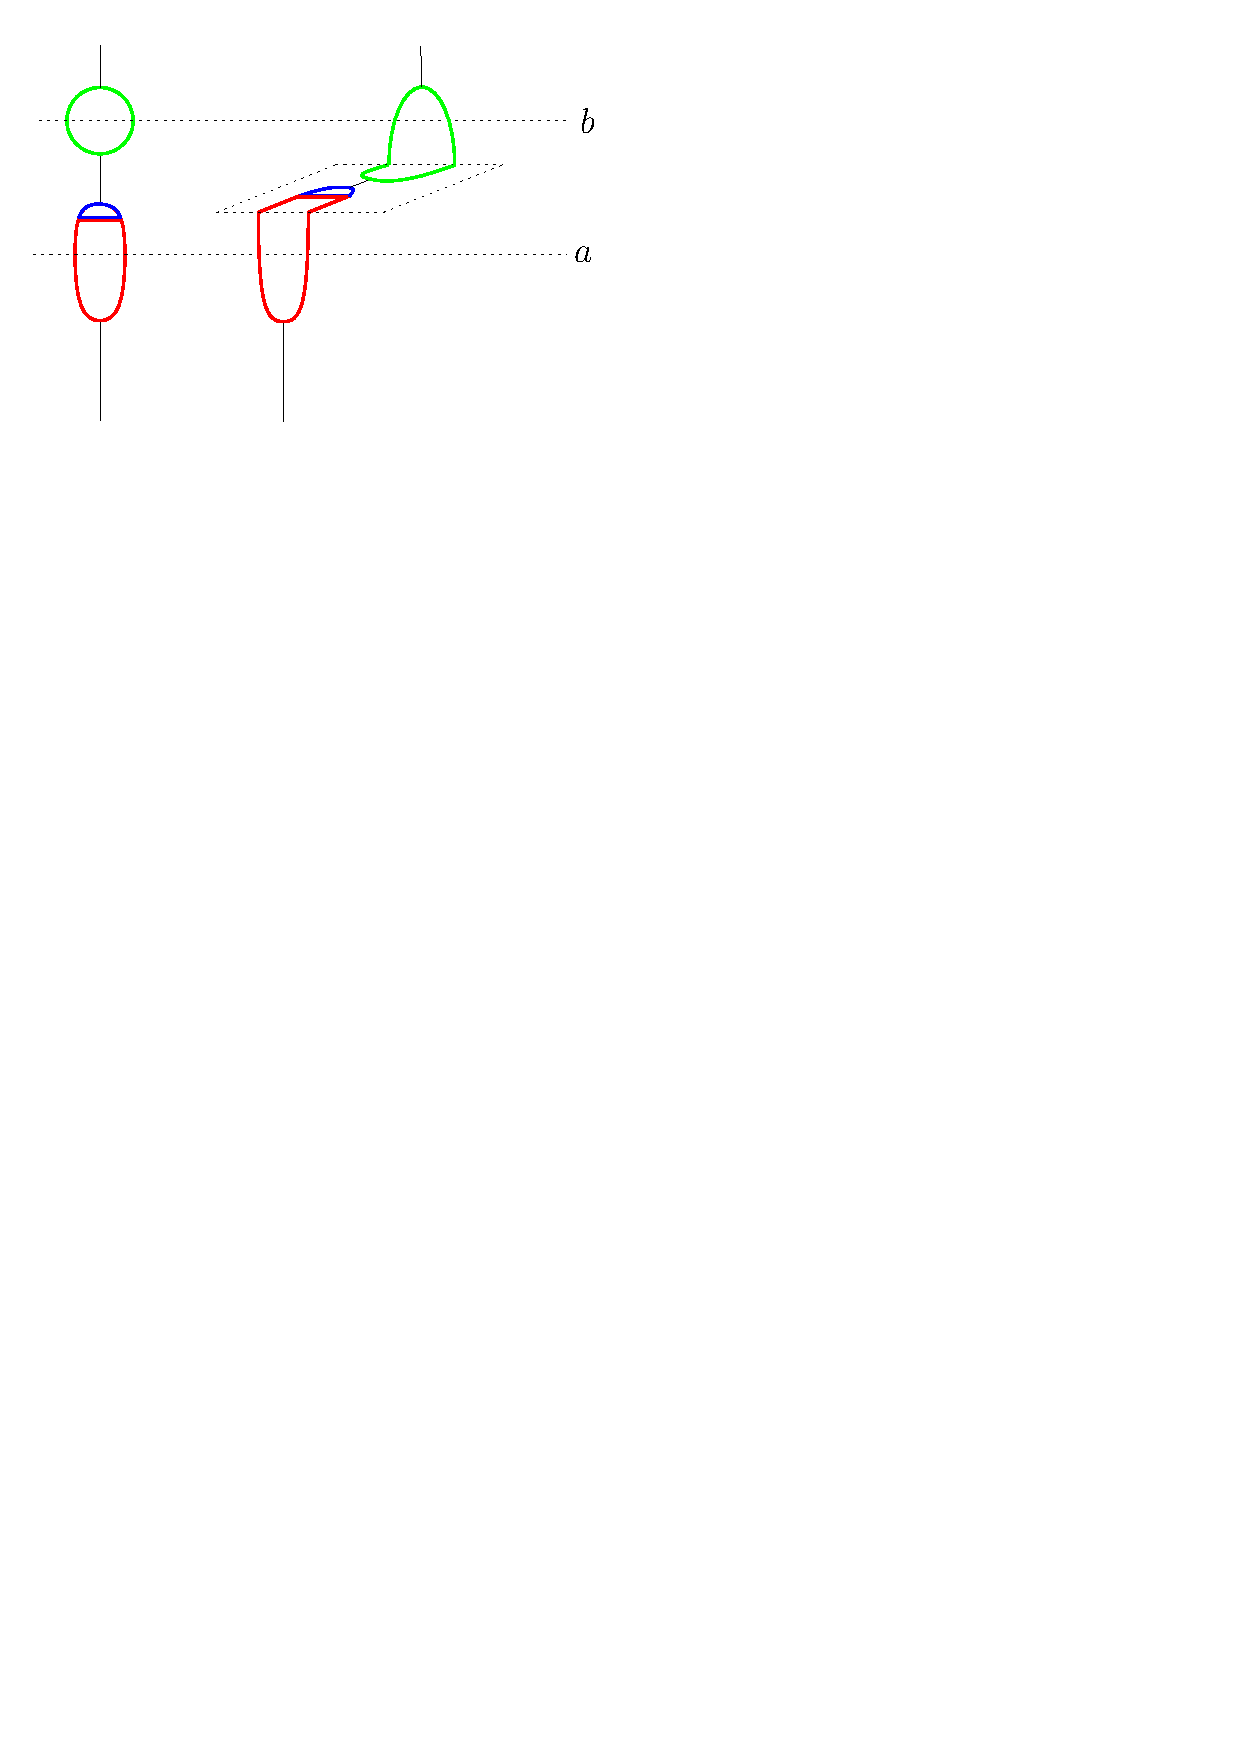
\includegraphics[height=4cm]{figures/MergeSpace}\ \ \ 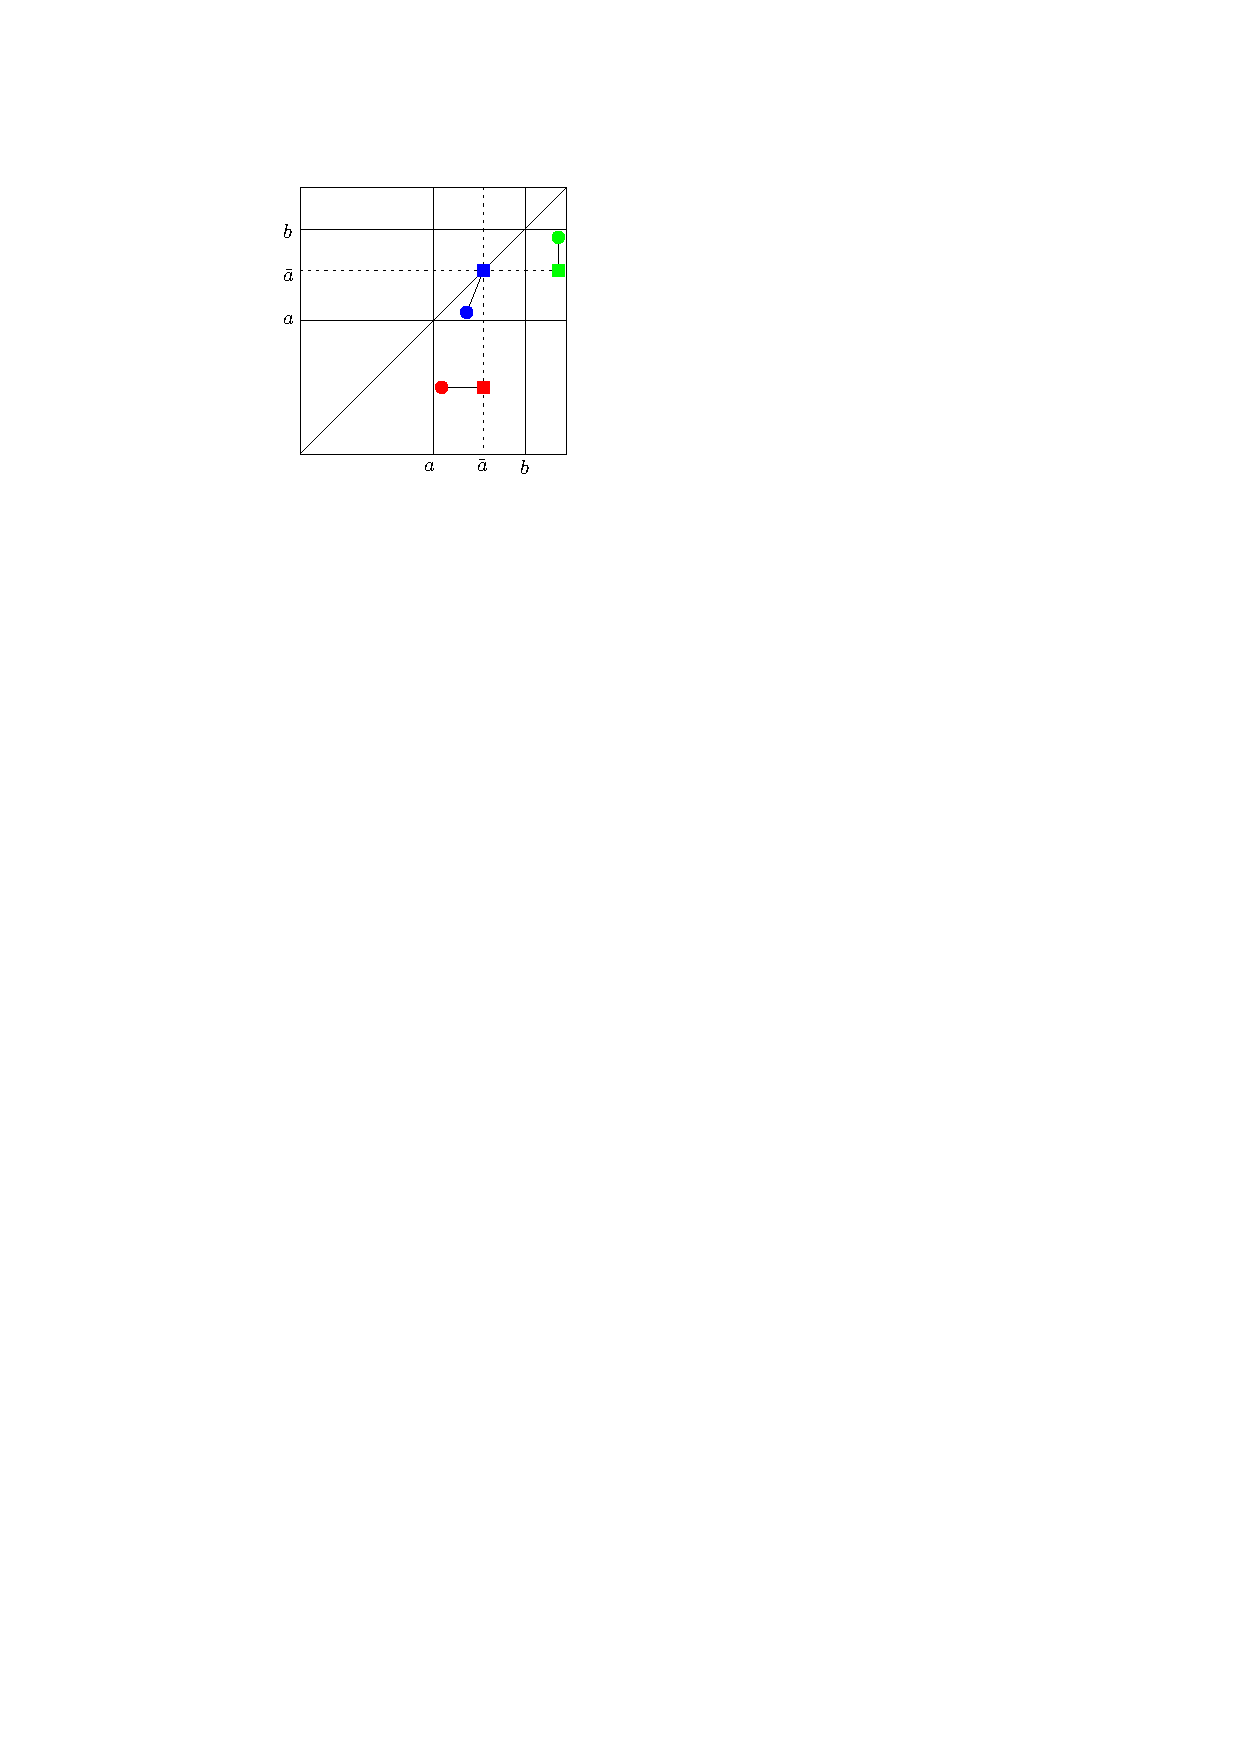
\includegraphics[width = 4cm]{figures/MergePD}
\caption[Merge]{\label{fig:mergespace} Left: Effect of a Merge on a telescope. %Middle: Effect on the corresponding Reeb graph. 
Right: Effect on the corresponding extended persistence diagram. 
Points before the Merge are disks while points after the Merge are squares.}
\end{center}\end{figure}
%
See the left panel of Figure~\ref{fig:mergespace} for an illustration.
%
\paragraph*{Merge for persistence diagrams.} 
Similarly, we define the Merge between $a,b$ on an extended persistence diagram~$\Dg$ as the diagram $\Merge_{a,b}(\Dg)$ given by
$\Merge_{a,b}(x,y)=({\bar x},{\bar y})$, where:
%
\[
{\bar x}=\left\{ \begin{array}{ll} x\text{ if }x\notin[a,b] \\ {\bar a}\text{ otherwise } \end{array} \right.
\text{ and }
{\bar y}=\left\{ \begin{array}{ll} y\text{ if }y\notin[a,b] \\ {\bar a}\text{ otherwise } \end{array} \right.
\]
%
Points in the strips $x\in[a,b]$, $y\in[a,b]$ are snapped to the lines
$x=\bar{a}$ and $y=\bar{a}$ respectively.  See the right panel of
Figure~\ref{fig:mergespace}.  See also the first intermediate points
along the trajectories of the red points in
Figure~\ref{fig:pdTRANS} for another illustration on extended
persistence diagrams.  

\paragraph*{Commutativity of the operators.} We now prove %in Lemma~\ref{lem:mergeprop} 
that extended persistent homology commutes with this operator, i.e. $\Dg(\Merge)=\Merge(\Dg)$.

\begin{lem}
\label{lem:mergeprop}
Let $a\leq b$ and $T'=\Merge_{a,b}(T)$. 
Let $\pi_2':T'\rightarrow\R$ be the projection onto the second factor. Then, $\Dg(\pi_2')=\Merge_{a,b}(\Dg(\pi_2))$.
\end{lem}

\begin{proof}
We only study the sublevel sets of the functions, which means that we
only prove the result for the ordinary part of the diagrams.  The
proof is symmetric for superlevel sets, leading to the result for
the extended and the relative parts. %$\Ext$ and $\Rel$.

Assume $a_{i-1}<a\leq a_i\leq a_j\leq b<a_{j+1}$.  Given $x\leq y$, we
let $\Pi_{x,y}:H_*\left(T^{(-\infty,x]}\right)\rightarrow
      H_*\left(T^{(-\infty,y]}\right)$ and
    $\Pi'_{x,y}:H_*\left((T')^{(-\infty,x]}\right)\rightarrow
  H_*\left((T')^{(-\infty,y]}\right)$ be the homomorphisms induced by
inclusions.  Since $f$ is of Morse type, Lemma~\ref{lem:defret}
relates $\Pi'$ to $\Pi$ as follows (see Figure~\ref{fig:areas}):

\begin{equation}\label{eq:rel}
\Pi'_{x,y}=\left\{ \begin{array}{ll} \Pi_{x,y}\text{ if }x,y\notin[a,b]\text{ (green)} & \Pi_{x,a_{i-1}}\text{ if }x<a,y\in[a,\bar{a})\text{ (pink)} \\
					   \Pi_{a_{i-1},y}\text{ if }x\in[a,\bar{a}),y>b\text{ (blue)} & \Pi_{a_{i-1},a_j}\text{ if }x\in[a,\bar{a}),y\in[\bar{a},b]\text{ (orange)}\\
					   \Pi_{a_j,y}\text{ if }x\in[\bar{a},b],y>b\text{ (grey)} & \text{id}^*_{Y_{i-1}}\text{ if }x,y\in[a,\bar{a})\text{ (brown)} \\
					   \Pi_{x,a_j}\text{ if }x<a,y\in[\bar{a},b]\text{ (turquoise)} & \text{id}^*_{Y_j}\text{ if }x,y\in[\bar{a},b]\text{ (purple)} 
		\end{array} \right.
\end{equation}

%%%
\begin{figure}[h]
\begin{center}
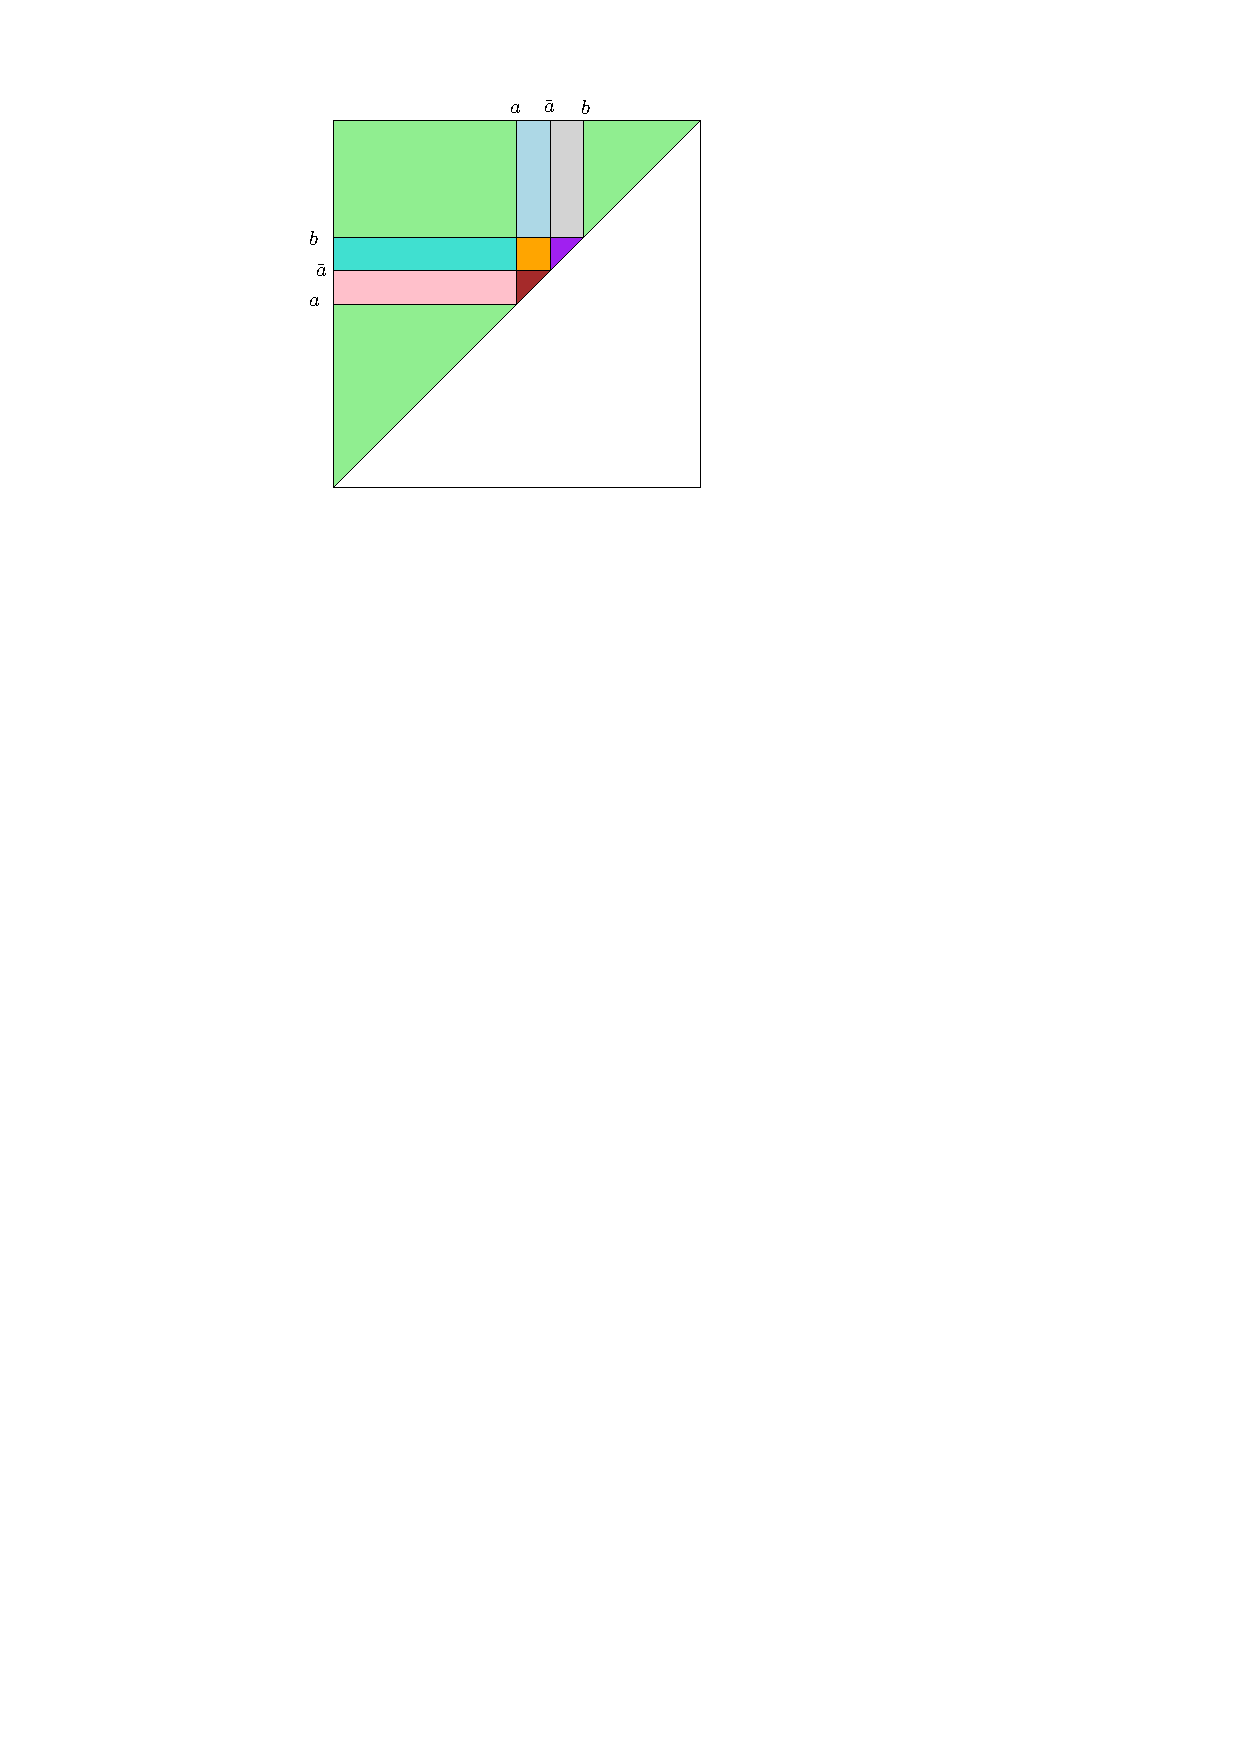
\includegraphics[width=7cm]{figures/MergeAreas}\ \ 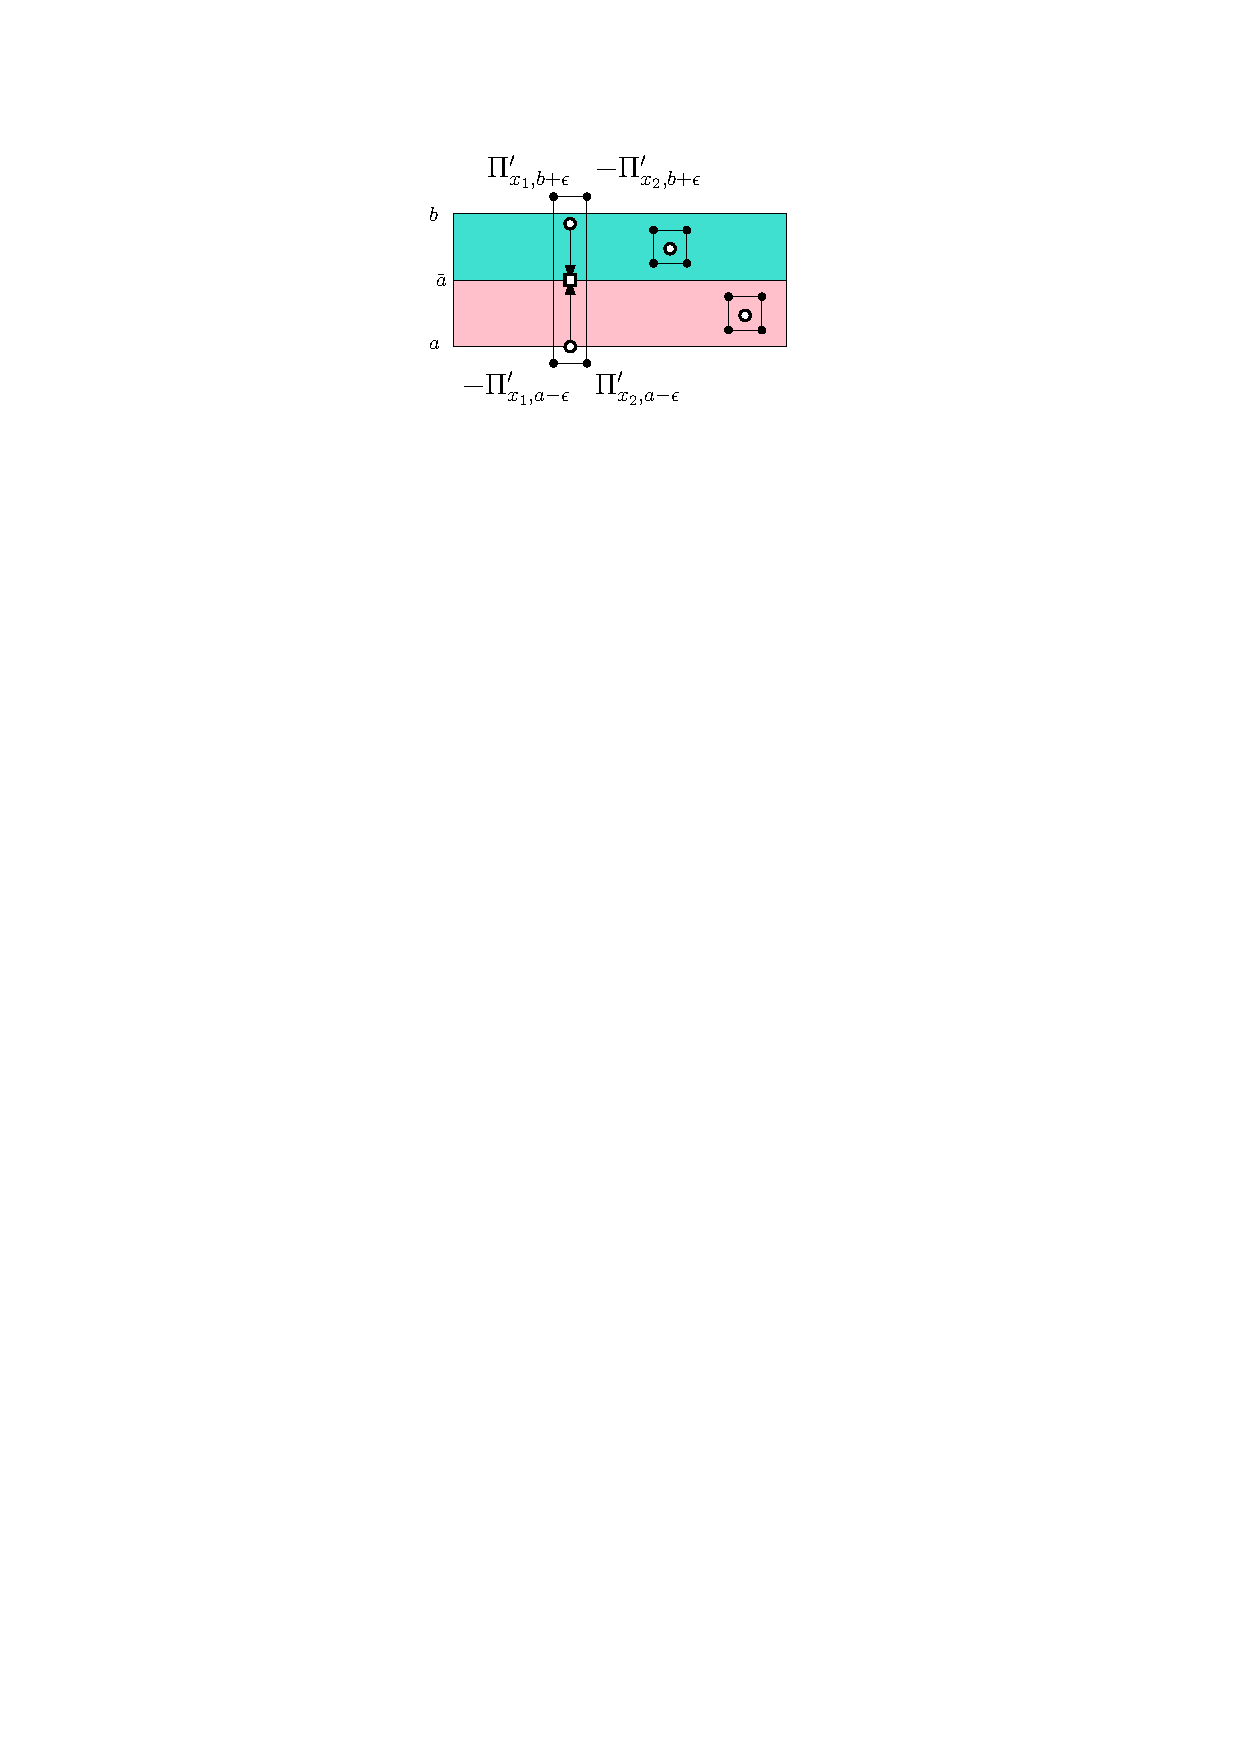
\includegraphics[width=8cm]{figures/PersMeasure}
\caption[Persistence measure for Merge]{\label{fig:areas}
%Example of a Merge between $a,b$.
Left: Areas of the extended persistence diagram used in the proof.
Right: Examples of the boxes we use to prove the result (circles represent points before the Merge, squares represent points after the Merge).
}
\end{center}
\end{figure}

The equality between the diagrams follows from these relations and the
inclusion-exclusion formula~(\ref{eq:pers_meas}).  Consider for
instance the case where the point $(x,y)\in\Dg(\pi_2)$ belongs to the
union $A$ of the pink and the turquoise areas.  One can select two
abscissae $x_1<x<x_2$ and an arbitrarily small $\epsilon>0$. Then, the
total multiplicity of the corresponding rectangle $R$ in $\Dg(\pi_2')$
(displayed in the right panel of Figure~\ref{fig:areas}) is given by:

\[ \text{mult}(R)=\text{rank}\ \Pi'_{x_2,a-\epsilon}-\text{rank}\ \Pi'_{x_2,b+\epsilon}+\text{rank}\ \Pi'_{x_1,b+\epsilon}-\text{rank}\ \Pi'_{x_1,a-\epsilon}. \]

The first relation in (\ref{eq:rel}) shows that $R$ has exactly the same multiplicity in $\Dg(\pi_2)$, since all its corners belong to the green area.
As this is true for arbitrarily small $\epsilon>0$, it means that $R'=R\cap A$  also has the same multiplicity in $\Dg(\pi_2)$ as in $\Dg(\pi'_2)$.
Now, if we pick a point inside $R'$ with an ordinate different than $\bar{a}$, we can compute its multiplicity in $\Dg(\pi'_2)$ 
by surrounding it with a box included in the turquoise area (if the ordinate is bigger than $\bar{a}$) or in the pink area (if it is smaller). 
Boxes in the turquoise area have multiplicity 
$\text{rank}\ \Pi'_{x_2,y_1}-\text{rank}\ \Pi'_{x_2,y_2}+\text{rank}\ \Pi'_{x_1,y_2}-\text{rank}\ \Pi'_{x_1,y_1}
=\text{rank}\ \Pi_{x_2,a_j}-\text{rank}\ \Pi_{x_2,a_j}+\text{rank}\ \Pi_{x_1,a_j}-\text{rank}\ \Pi_{x_1,a_j}=0$. 
Similarly, boxes in the pink area also have  multiplicity zero. Thus, all points of $R'$ in $\Dg(\pi'_2)$ have 
ordinate $\bar{a}$. Again, as it is true for $x_1,x_2$ as close to each other as we want, it means that $(x,y)$ 
is snapped to $(x,\bar{a})$ in $\Dg(\pi'_2)$. The treatment of the other areas in the plane is similar.

Now, if $[a,b]$ contains no critical values, then $\Pi'=\Pi$, so the result is clear.
\end{proof}



\subsection*{Split}
\label{sec:split}

Split operators split a critical value $a_i$ into two different ones $a_i-\e$ and $a_i+\e$. 

\begin{defin}[Split]\label{def:split}
Let $T$ be a telescope.
Let $a_i\in\Crit(T)$ and $\epsilon$ such that $$0\leq\epsilon<\displaystyle\min\{a_{i+1}-a_i,a_i-a_{i-1}\}.$$ 
The $\epsilon$-Split on $T$ at $a_i$ is the telescope $T'=\Split_{\epsilon,a_i}(T)$ given by:
%
\[~\hspace{-10mm}
\begin{array}{c}
...(Y_{i-1}\times[a_{i-1},a_i])\cup_{\psi_{i-1}}(X_i\times\{a_i\})\cup_{\phi_i}(Y_i\times[a_i,a_{i+1}])... \\
\rotatebox[origin=c]{270}{$\mapsto$}\\
...(Y_{i-1}\times[a_{i-1},a_i-\epsilon])\cup_{\psi_{i-1}^{a_i-\epsilon}}(X_i\times\{a_i-\epsilon\})
\cup_{{\rm id}}(X_i\times[a_i-\epsilon,a_i+\epsilon])\cup_{{\rm id}}(X_i\times\{a_i+\epsilon\})
\cup_{\phi_i^{a_i+\epsilon}}(Y_i\times[a_i+\epsilon,a_{i+1}])...
\end{array}
\]
%
\end{defin}

See the left panel of Figure~\ref{fig:splitspace} for an
illustration.  
%
\begin{figure}[h!]\begin{center}
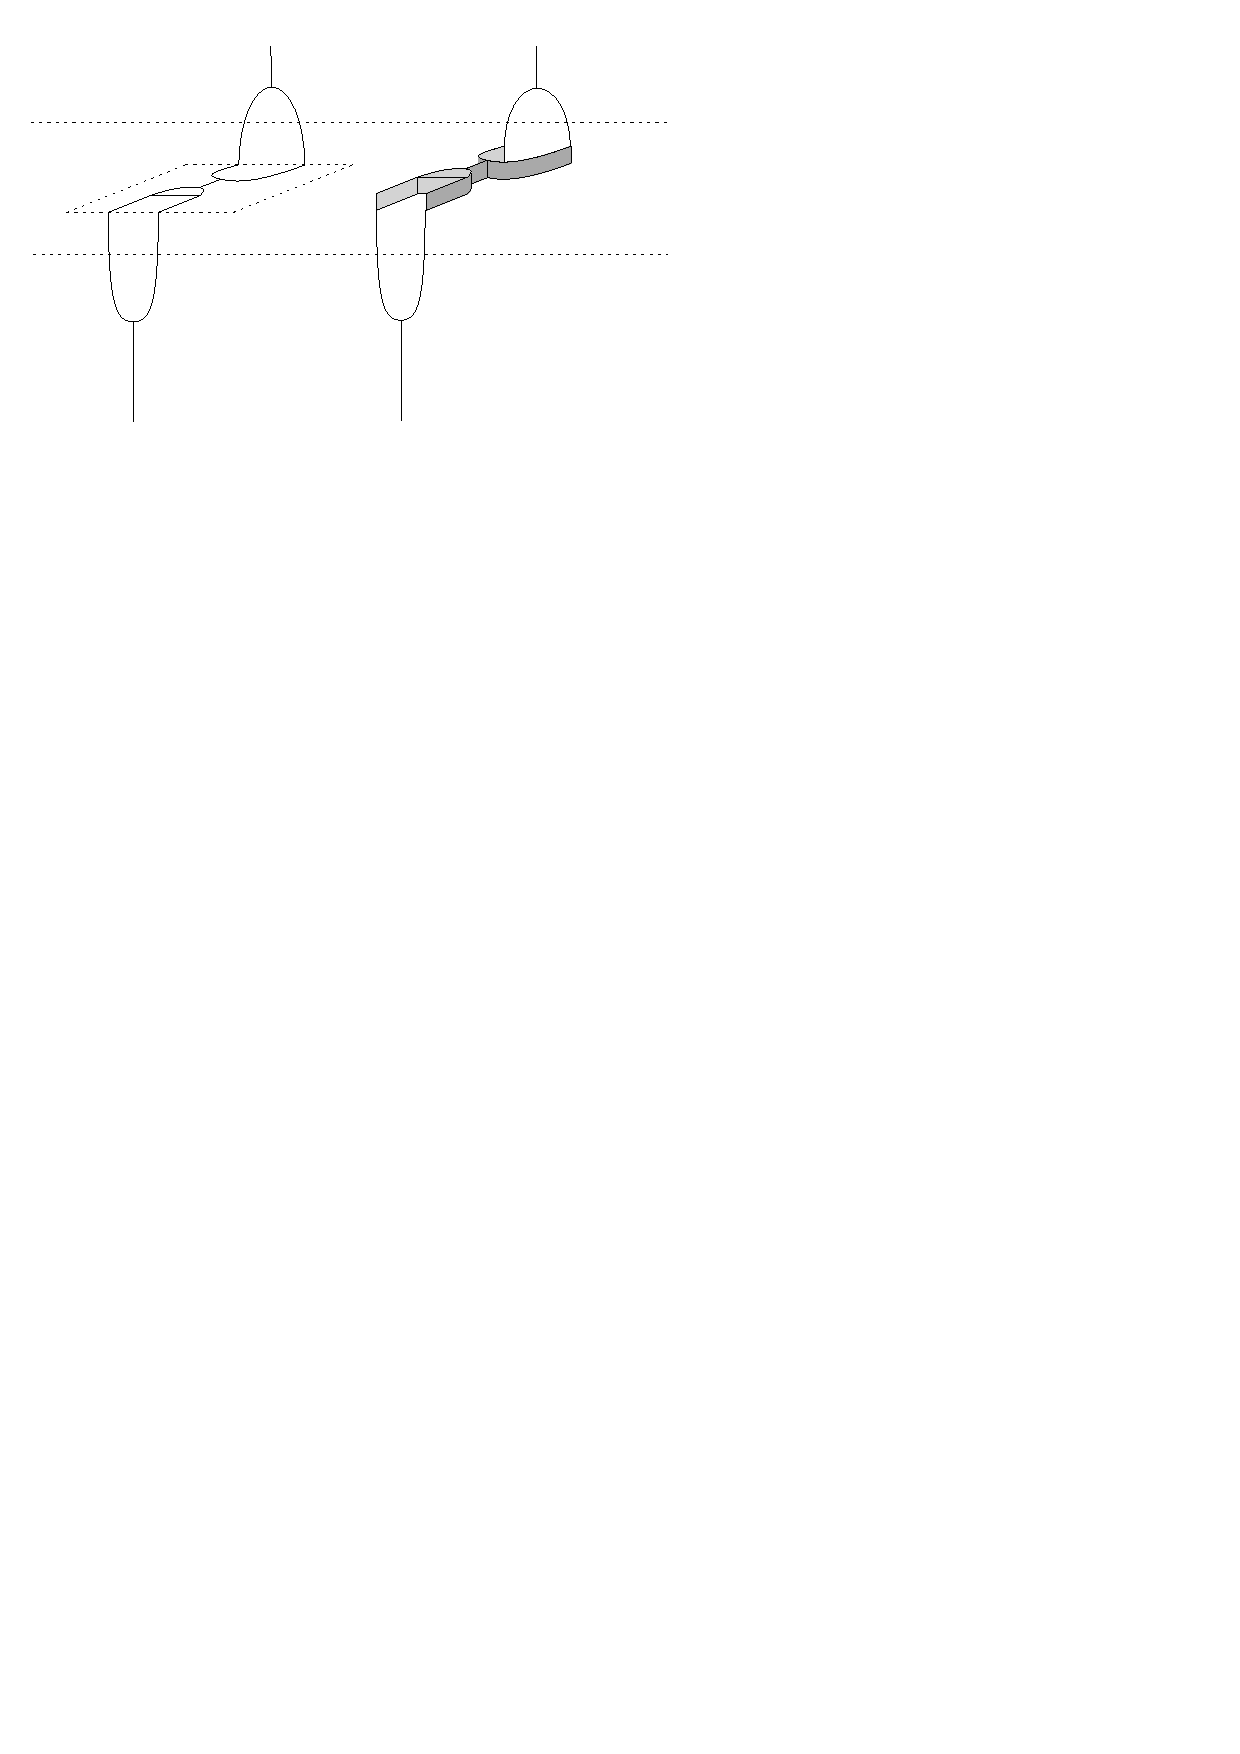
\includegraphics[height=4cm]{figures/SplitSpace}\ \ \ 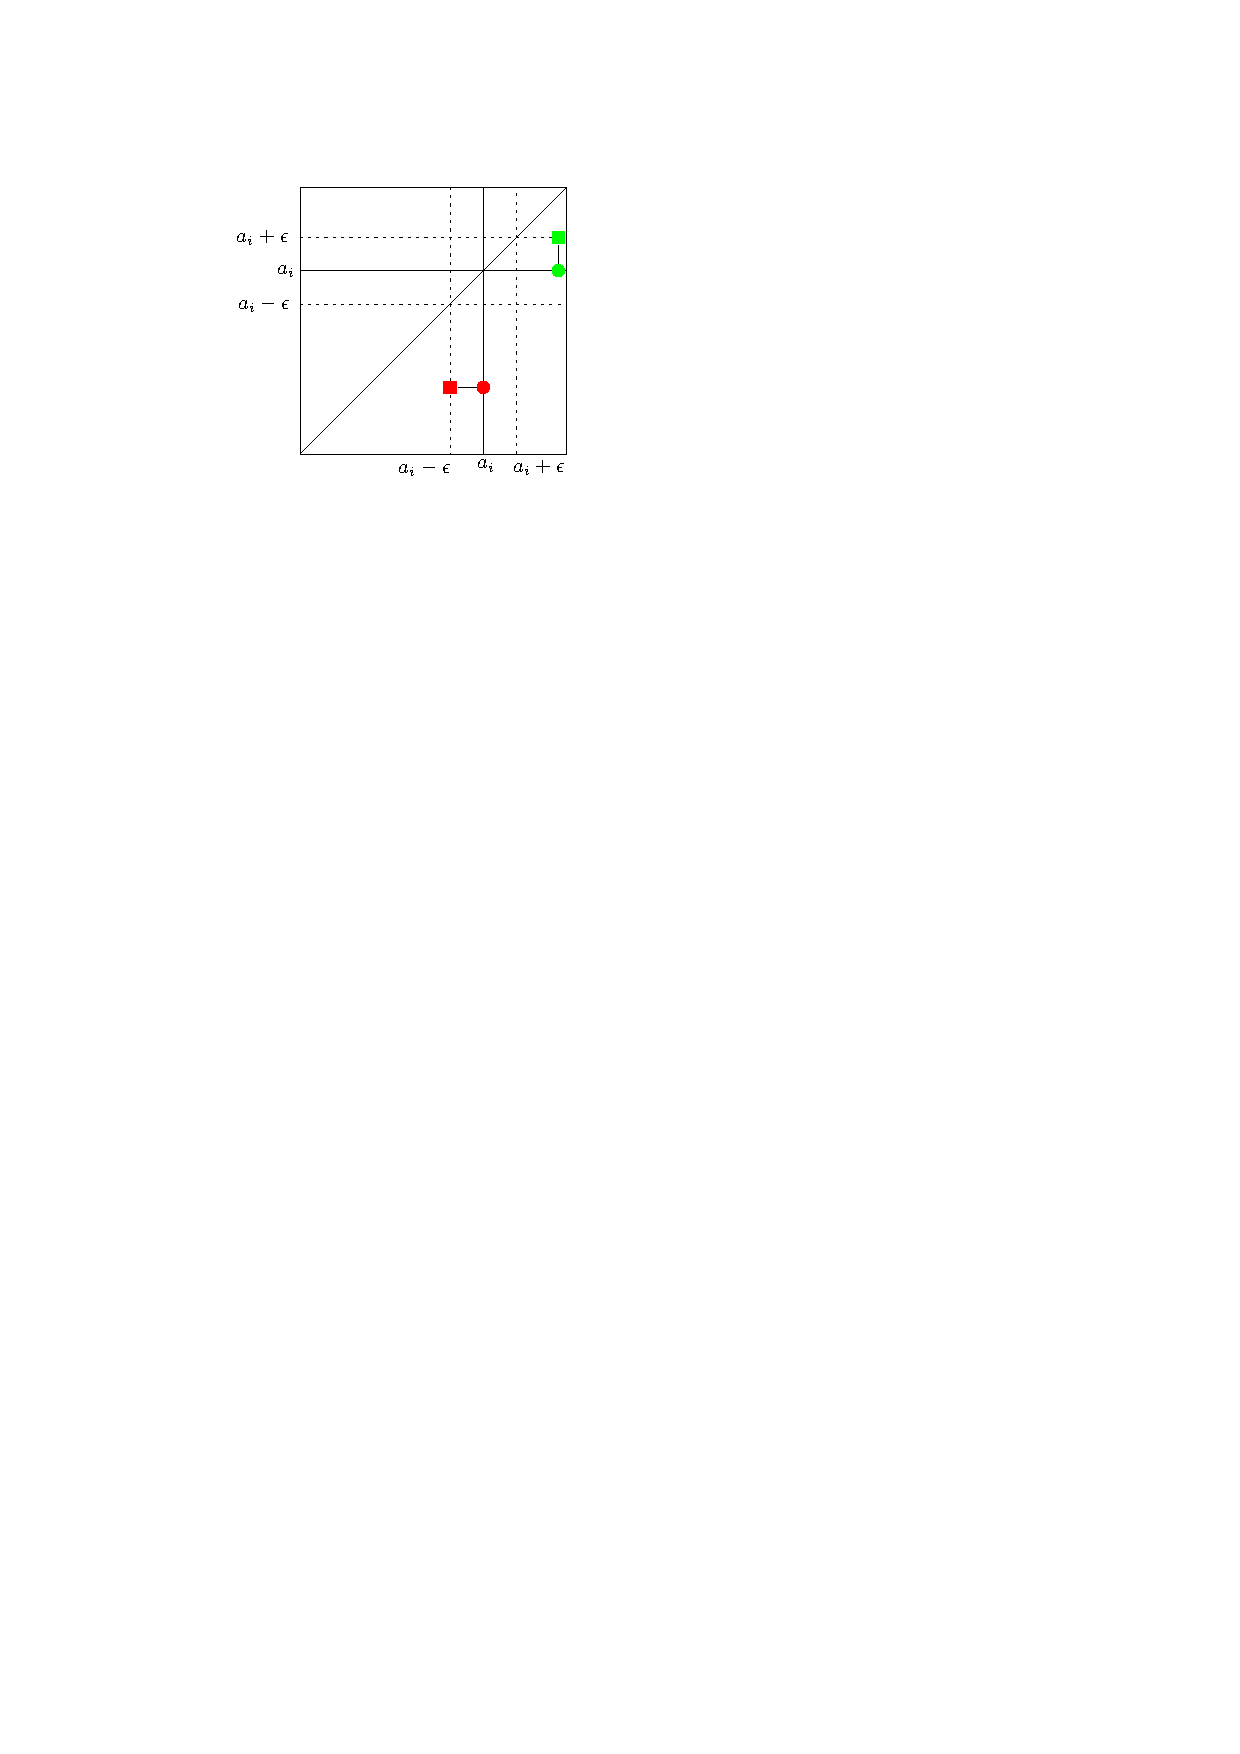
\includegraphics[width = 4cm]{figures/SplitPD}
\caption[Split]{\label{fig:splitspace} Left: Effect of a Split on a telescope. %Middle: Effect on the corresponding Reeb graph. 
Right: Effect on the corresponding extended persistence diagram. Points before the Split are disks while points after the Split are squares.}
\end{center}\end{figure}
%




\paragraph*{Down- and up-forks.} Splits create particular critical values called {\em down-} and {\em up-forks}.
Intuitively, Split operations allow to distinguish between all possible types of
changes in 0- and 1-dimensional homology of the sublevel and superlevel sets, namely: 
union of two connected components, creation of a connected component, destruction of a connected component,
and separation of a connected component. Unions and creations occur at down-forks while separations and destructions occur at up-forks.
See Figure~\ref{fig:split} for an illustration. We formalize and prove this intuition in Lemma~\ref{lem:dict}.

\begin{defin}
A critical value $a_i\in\Crit(T)$ is called an \emph{up-fork} if $\psi_{i-1}$ is an homeomorphism, and
it is called a \emph{down-fork} if $\phi_i$ is a homeomorphism.
\end{defin}

%%%
\begin{figure}[h]
\begin{center}
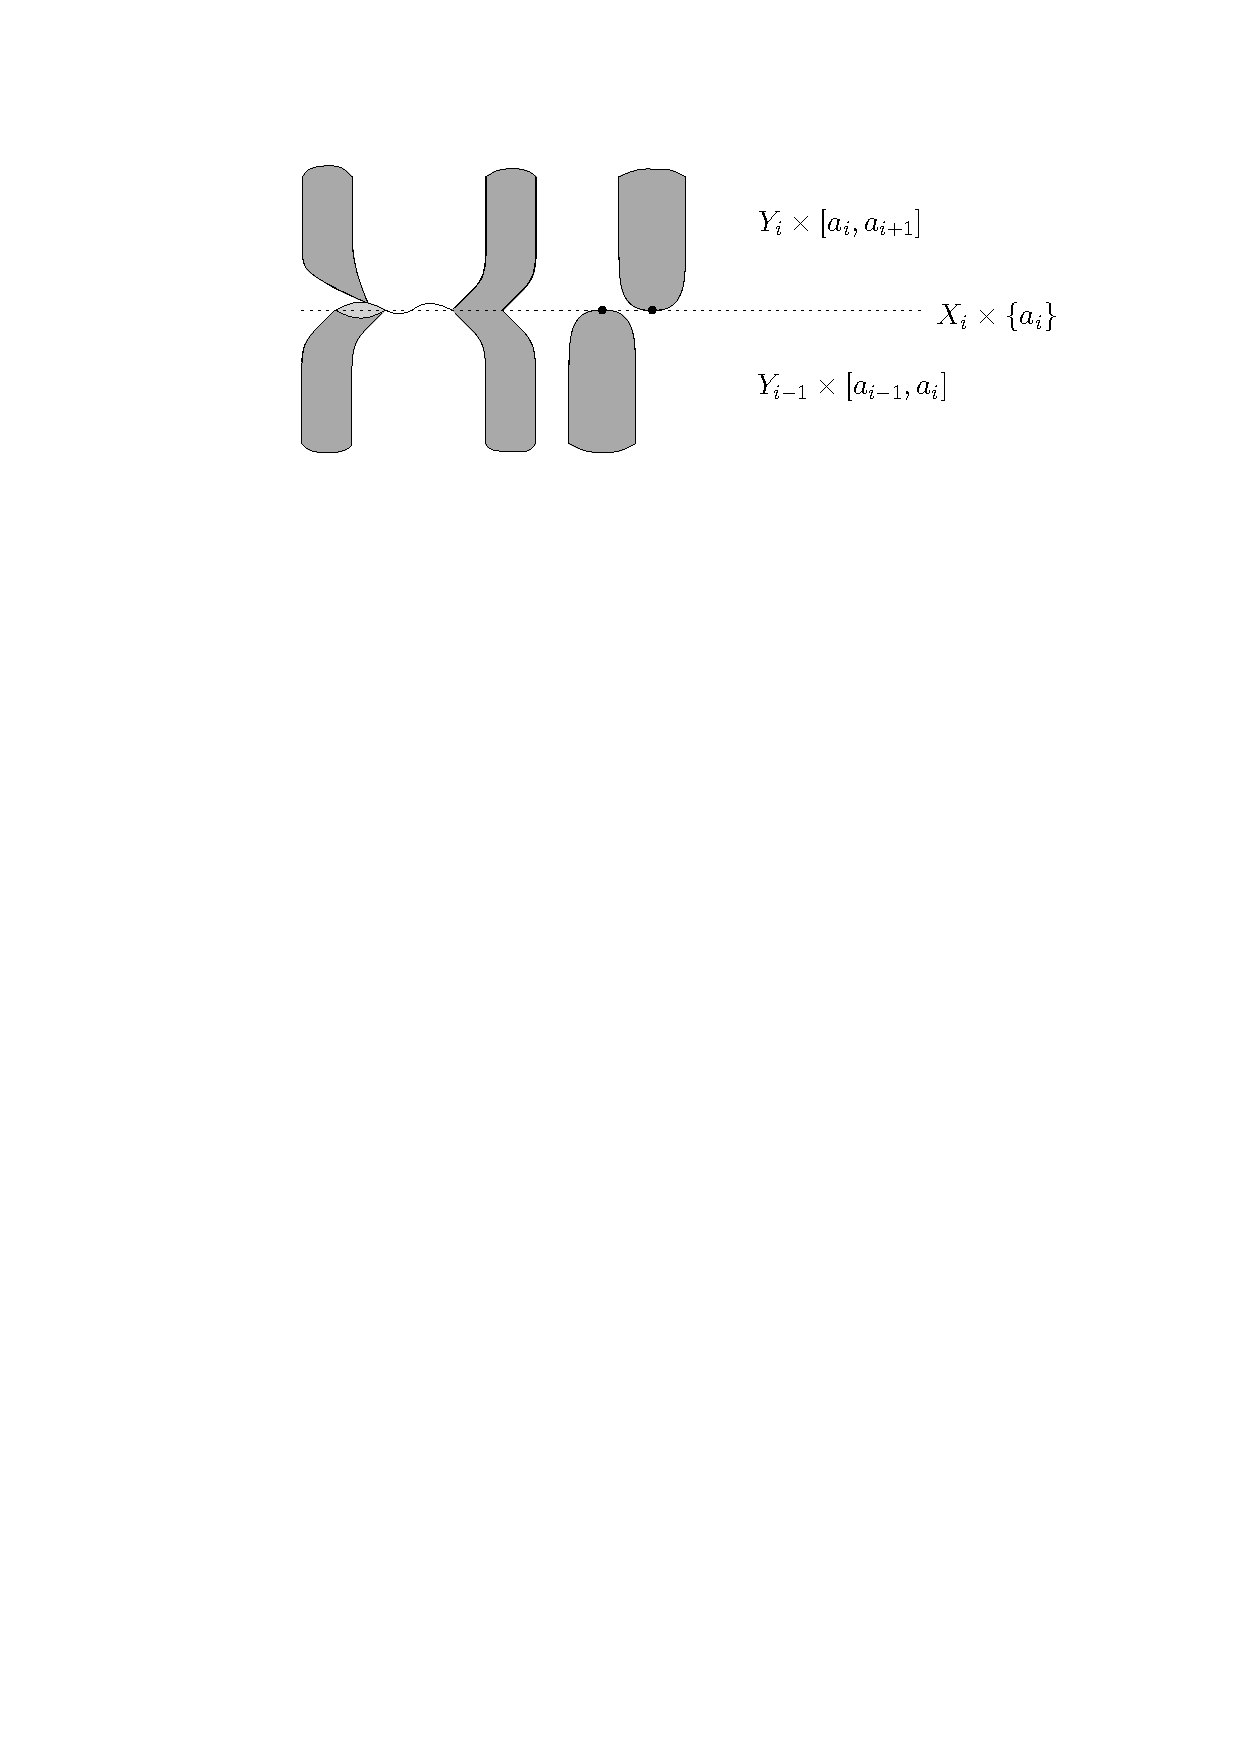
\includegraphics[width=7cm]{figures/SplitBefore}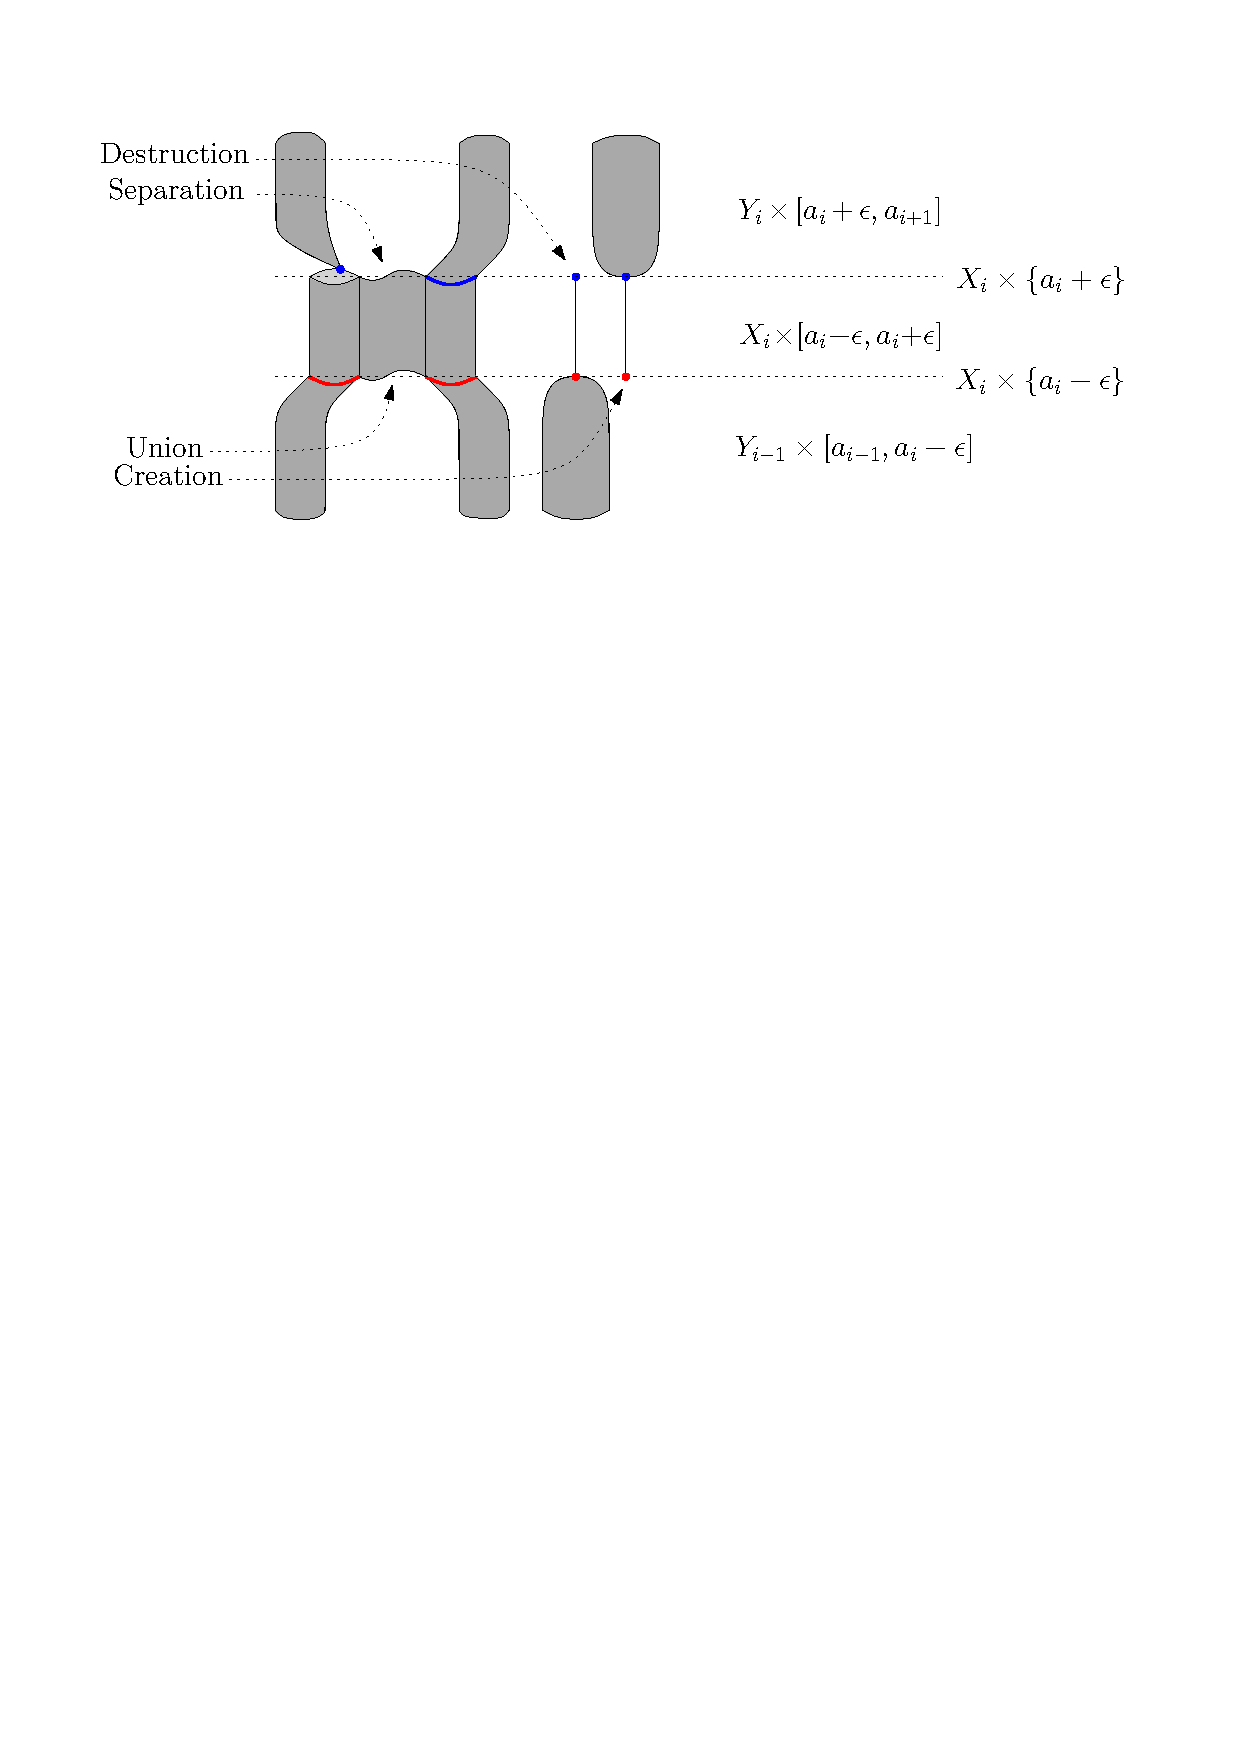
\includegraphics[width=9cm]{figures/SplitAfter}
\caption[Up- and down-forks]{\label{fig:split}
Left and right panels display the space before and after a Split respectively.
Subsets of $X_i$ that are colored in red and blue correspond to $\im(\pi_1\circ\psi_{i-1})$
and $\im(\pi_1\circ\phi_i)$ respectively.}
\end{center}
\end{figure}

Since the attaching maps introduced by the Split are
identity maps, we have the following lemma:
\begin{lem}\label{lem:classif}
The critical values $a_i-\epsilon$ and $a_i+\epsilon$ created with $\Split$ are down- and up-forks respectively.
\end{lem}

The next lemma is a direct consequence of the existence and continuity
of $\phi_i^{-1}$ (resp. $\psi_{i-1}^{-1}$) when $a_i\in\Crit(T)$ is a
down-fork (resp. up-fork):

\begin{lem}\label{lem:forks} Let $a_i\in\Crit(T)$. If $a_i$ is an up-fork, then
    $T^{(-\infty,a_i]}$ deform retracts onto
    $T^{(-\infty,\alpha]}$ for all $\alpha \in
  (a_{i-1},a_i]$. %Similarly, i
    If $a_i$ is a down-fork, then
    $T^{[a_i,+\infty)}$ deform retracts onto
      $T^{[\alpha,+\infty)}$ for all $\alpha \in [a_i,a_{i+1})$.
\end{lem}

Now we can prove the previous intuition concerning down- and up-forks correct:

\begin{lem}\label{lem:dict}
Let $a_i\in\Crit(T)$.
If $a_i$ is an up-fork, then it can only be the birth time of relative cycles and the death time of relative and extended cycles in $\Dg(\pi_2)$.
If $a_i$ is a down-fork, then it can only be the birth time of ordinary and extended cycles and the death time of ordinary cycles in $\Dg(\pi_2)$.
\end{lem}

\begin{proof}
Let $0\leq \epsilon,\epsilon' < \min\{a_{i+1}-a_i,a_i-a_{i-1}\}$. Consider the extended persistence module of $\pi_2$:
%
\[
\begin{array}{lllllllll}
... & \longrightarrow & H_*\left(T^{(-\infty,a_i-\epsilon]}\right) & \longrightarrow & H_*\left(T^{(-\infty,a_i]}\right) & \longrightarrow & H_*\left(T^{(-\infty,a_i+\epsilon']}\right) &\longrightarrow & ... \\[1em]
... & \longrightarrow & H_*\left(T,T^{[a_i+\epsilon',+\infty)}\right) & \longrightarrow & H_*\left(T,T^{[a_i,+\infty)}\right) & \longrightarrow & H_*\left(T,T^{[a_i-\epsilon,+\infty)}\right) & \longrightarrow & ...
\end{array}
\]
%
If $a_i$ is an up-fork, then the composition
$H_*(T^{(-\infty,a_i-\epsilon]}) \to
        H_*(T^{(-\infty,a_i+\epsilon']})$ is an
      isomorphism since $T^{(-\infty,a_i+\epsilon']}$ deform
    retracts onto $T^{(-\infty,a_i-\epsilon]}$ by
      Lemmas~\ref{lem:defret} and \ref{lem:forks}. As
      $\epsilon,\epsilon'$ can be chosen arbitrarily small, there cannot be
      any creation of ordinary or extended cycle at $a_i$. There also
      cannot be any destruction of ordinary cycle.

Similarly, if $a_i$ is a down-fork, then the composition
$H_*(T,T^{[a_i+\epsilon',+\infty)}) \to
  H_*(T,T^{[a_i-\epsilon,+\infty)})$ is an isomorphism
    since $T^{[a_i-\epsilon,+\infty)}$ deform retracts onto
      $T^{[a_i+\epsilon',+\infty)}$. Again, there cannot be any
        destruction of extended or relative cycle at $a_i$. There also
        cannot be any creation of relative cycle.
\end{proof}

\paragraph*{Split for persistence diagrams.}
Similarly, we define the $\epsilon$-Split at $a_i$ on a
diagram~$\Dg$ as the diagram $\Split_{\epsilon,a_i}(\Dg)$ given by
$\Split_{\epsilon,a_i}(x,y)= (\bar x, \bar y)$, where:
%
\[
\bar x = \left\{\begin{array}{l}
x\ \mbox{if}\ x\neq a_i\\
a_i+\epsilon\ \mbox{if}\ 
x=a_i\ \mbox{and}\ 
(x,y)\in\Rel\\
a_i-\epsilon\ \mbox{if}\ 
x=a_i\ \mbox{and}\ 
(x,y)\notin\Rel
\end{array}\right.
\ \mbox{and}\ 
\bar y = \left\{\begin{array}{l}
y\ \mbox{if}\ y\neq a_i\\
a_i-\epsilon\ \mbox{if}\ 
y=a_i\ \mbox{and}\ 
(x,y)\in\Ord\\
a_i+\epsilon\ \mbox{if}\ 
y=a_i\ \mbox{and}\ 
(x,y)\notin\Ord
\end{array}\right.
\]
%
Points located on the lines $x,y=a_i$ are snapped to the lines
$x,y=a_i\pm\epsilon$ according to their type. Note that the definition
of $\Split_{\epsilon,a_i}(\Dg)$ assumes implicitly that $\Dg$ contains no
point within the horizontal and vertical bands $[a_i-\epsilon, a_i)\times\R$, 
$(a_i, a_i+\epsilon]\times\R$, $\R\times [a_i-\epsilon, a_i)$ and 
$\R\times (a_i, a_i+\epsilon]$, which is the
case under the assumptions of Definition~\ref{def:split}.
See the right panel of Figure~\ref{fig:splitspace} for an
illustration. See also the second intermediate points along the
trajectories of the red points in Figure~\ref{fig:pdTRANS} for another
illustration on extended persistence diagrams. 

\paragraph*{Commutativity of the operators.} We now prove %in Lemma~\ref{lem:splitprop} 
that extended persistent homology commutes with this operator, i.e.
$\Dg(\Split)=\Split(\Dg)$.

\begin{lem}
\label{lem:splitprop}
Let $a_i\in\Crit(T)$.
Let $0<\epsilon<\displaystyle\min\{a_{i+1}-a_i,a_i-a_{i-1}\}$, 
$T'=\Split_{\epsilon,a_i}(T)$ and $\pi_2':T'\rightarrow\R$ the projection 
onto the second factor. Then, $\Dg(\pi_2')=\Split_{\epsilon,a_i}(\Dg(\pi_2))$.
\end{lem}

\begin{proof}
Note that $T=\Merge_{a_i-\epsilon,a_i+\epsilon}(T')$. Hence, by
Lemma~\ref{lem:mergeprop},  $\Dg(\pi_2)$ can be obtained from $\Dg(\pi_2')$ 
with $\Dg(\pi_2)=\Merge_{a_i-\epsilon,a_i+\epsilon}(\Dg(\pi_2'))$.  Note also that
$\pi'_2$ has no critical value within the open interval
$(a_i-\epsilon,a_i+\epsilon)$, so $\Dg(\pi'_2)$ has no point within the
horizontal and vertical bands $\R\times (a_i-\e, a_i+\e)$ and
$(a_i-\e, a_i+\e)\times\R$. Finally, Lemma~\ref{lem:classif} ensures
that $a_i+\epsilon,a_i-\epsilon$ are up- and down-forks respectively,
so Lemma~\ref{lem:dict} tells us exactly where the preimages of the
points of $\Dg(\pi_2)$ through the Merge are located depending on
their type.
\end{proof}

\subsection*{Shift}
\label{sec:shift}

Shift operators translate critical values.

\begin{defin}[Shift]\label{def:shift}
Let $T$ be a telescope.
Let $a_i\in\Crit(T)$ and $\epsilon$ such that 
$$0\leq|\epsilon|<\displaystyle\min\{a_{i+1}-a_i,a_i-a_{i-1}\}.$$ 
The $\epsilon$-Shift on $T$ at $a_i$ is the telescope $T'=\Shift_{\epsilon,a_i}(T)$ given by:
%
\[\begin{array}{c}
...(Y_{i-1}\times[a_{i-1},a_i])\cup_{\psi_{i-1}}(X_i\times\{a_i\})\cup_{\phi_i}(Y_i\times[a_i,a_{i+1}])...\\
\rotatebox[origin=c]{270}{$\mapsto$}\\
...(Y_{i-1}\times[a_{i-1},a_i+\epsilon])\cup_{\psi_{i-1}^{a_i+\epsilon}}(X_i\times\{a_i+\epsilon\})\cup_{\phi_i^{a_i+\epsilon}}(Y_i\times[a_i+\epsilon,a_{i+1}])...
\end{array}\]
%
\end{defin}

See the left panel of Figure~\ref{fig:shiftspace} for an illustration. 

\begin{figure}[h!]\begin{center}
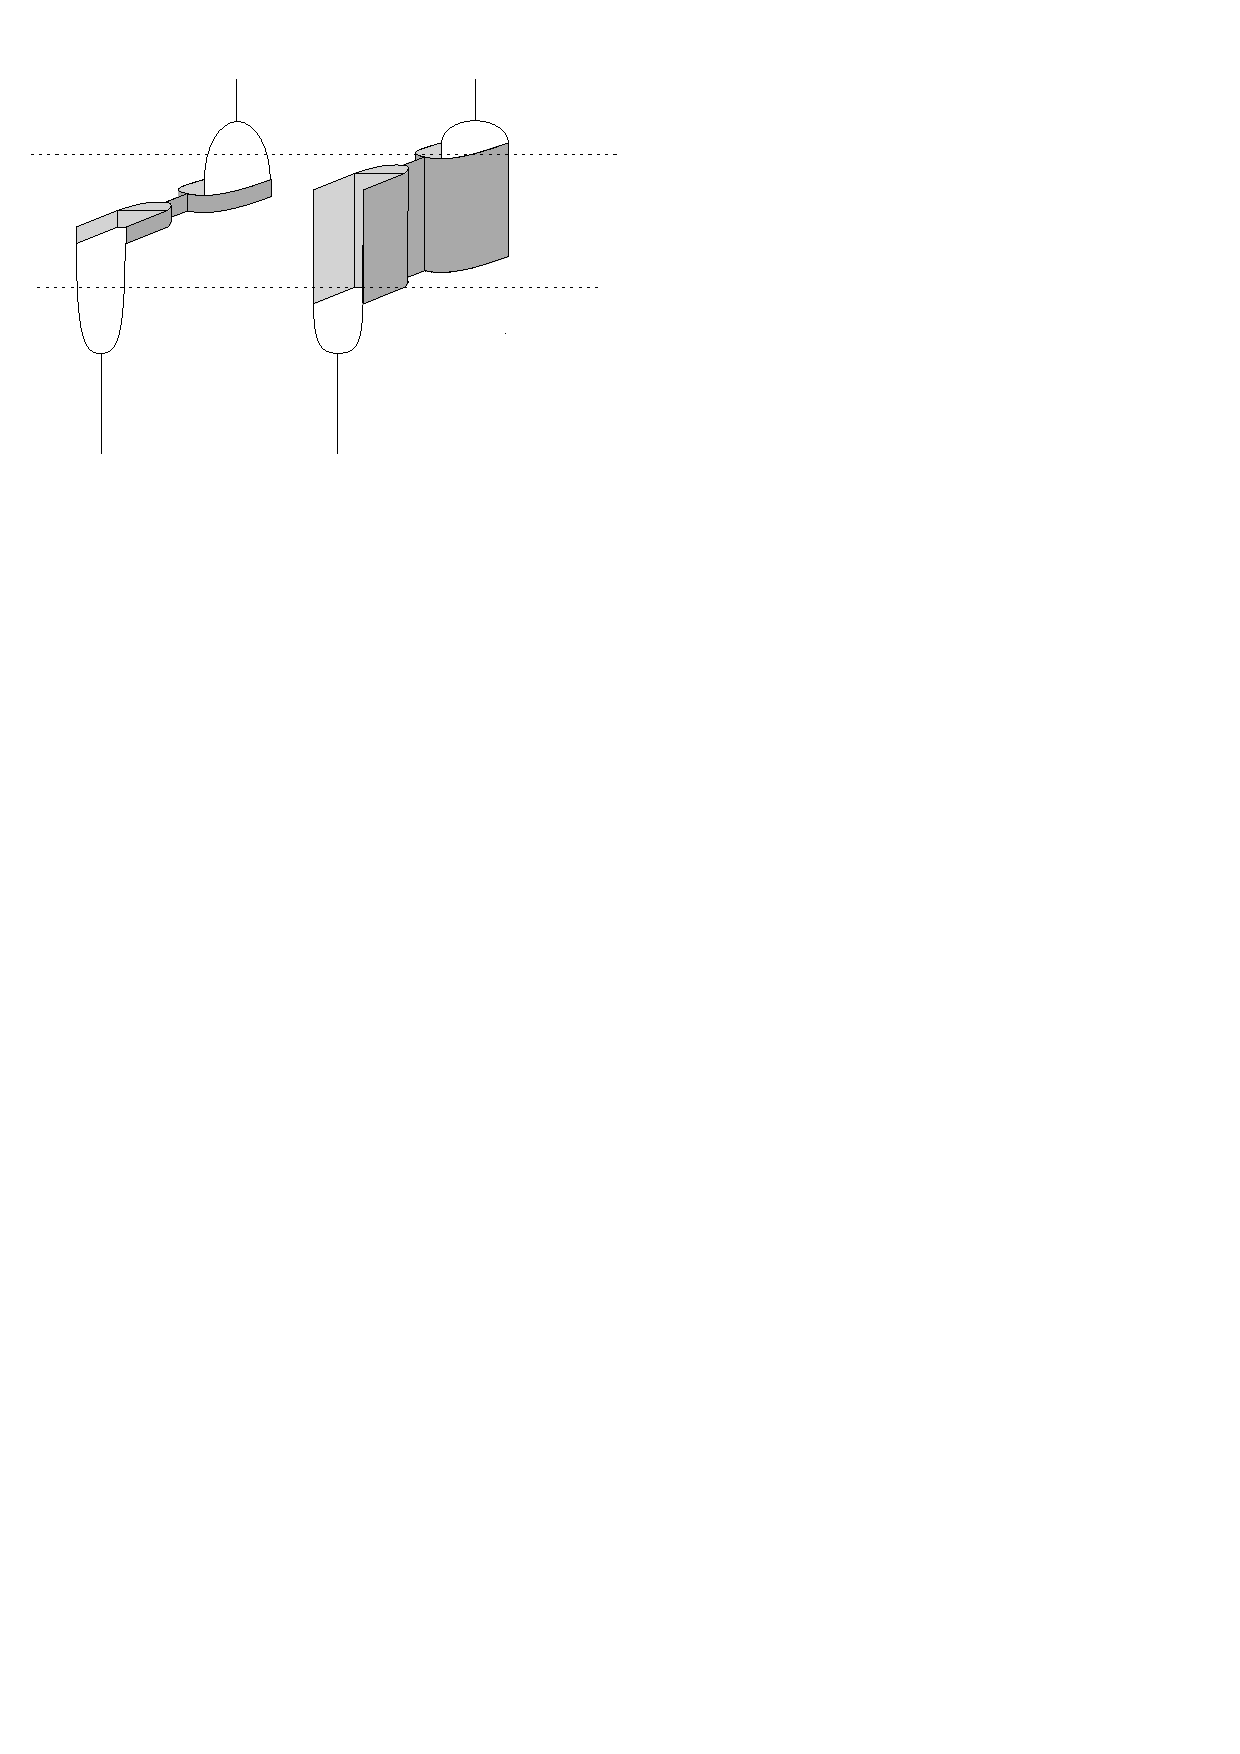
\includegraphics[height=4cm]{figures/ShiftSpace}\ \ \ 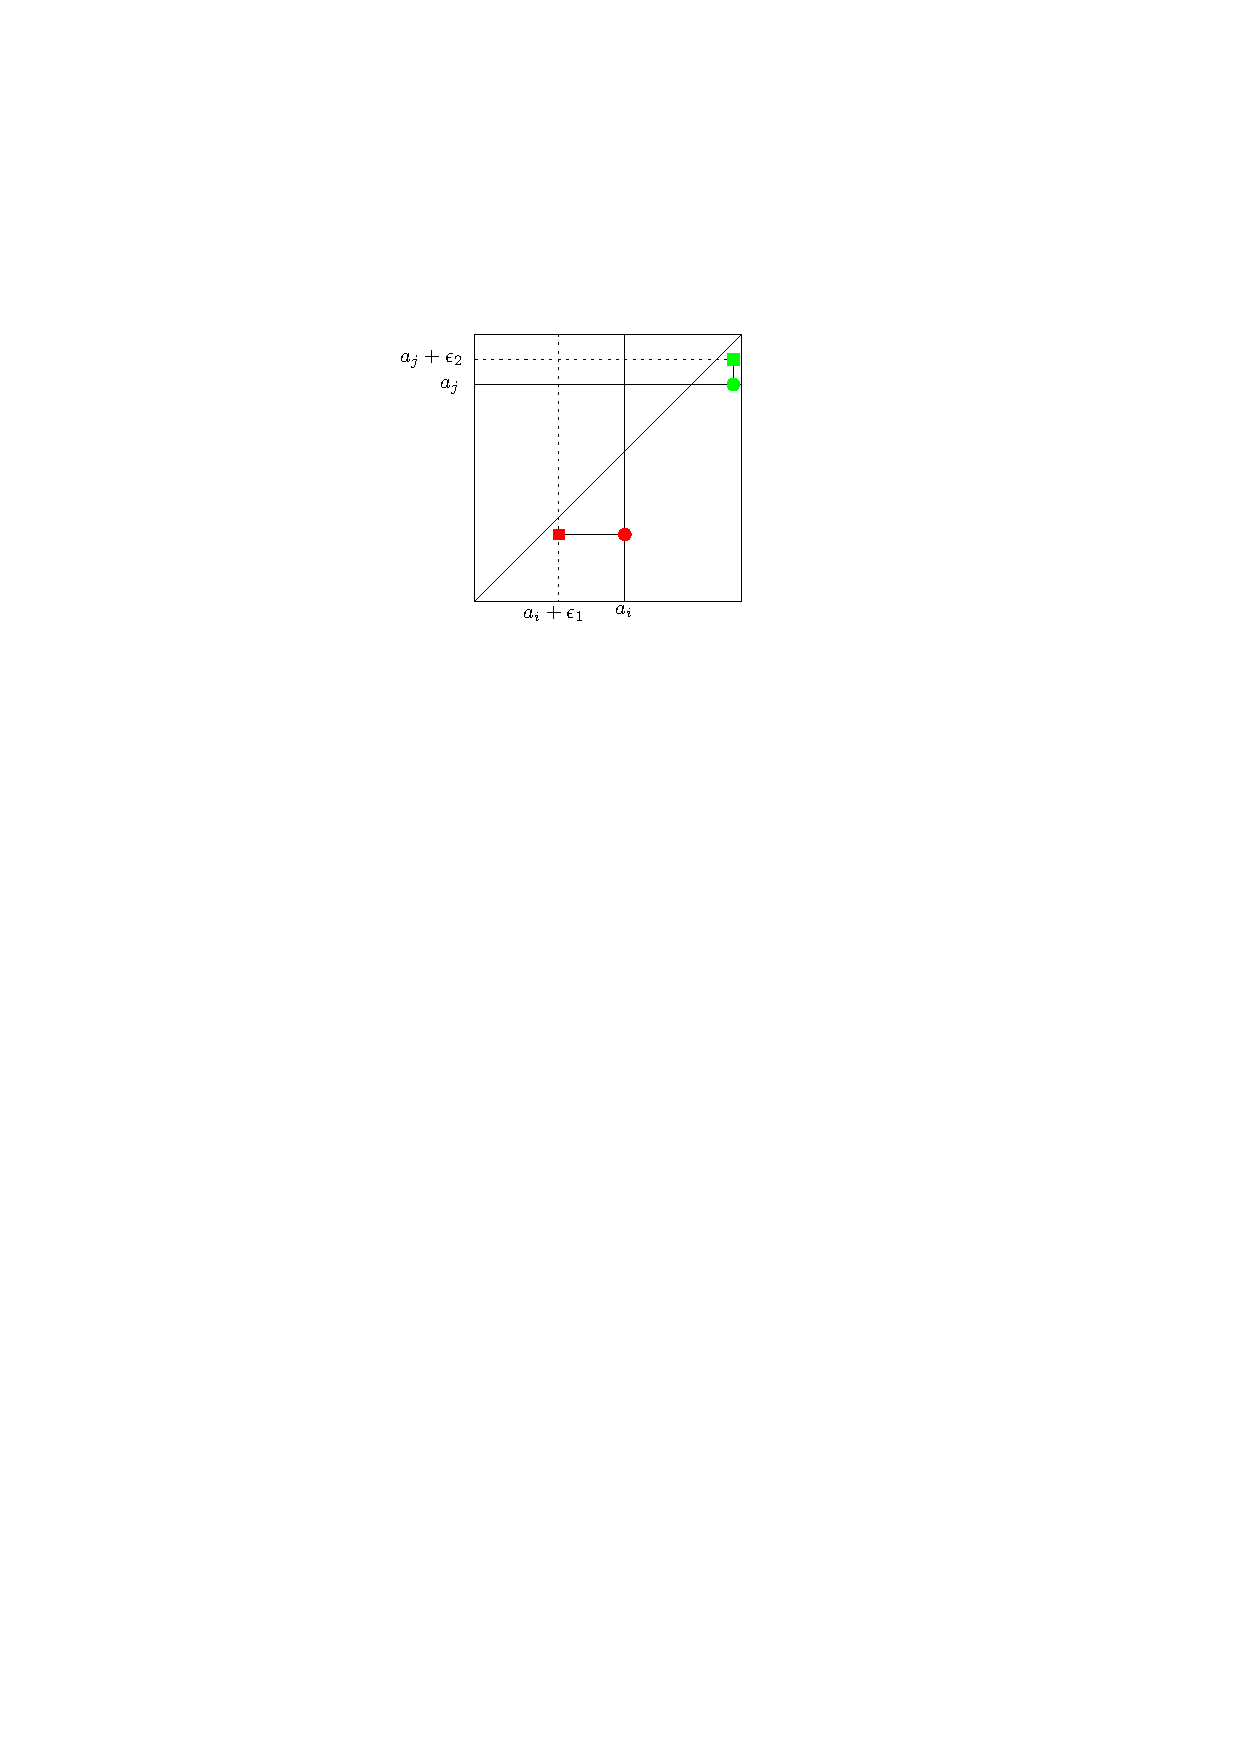
\includegraphics[width = 4cm]{figures/ShiftPD}
\caption[Shift]{\label{fig:shiftspace} Left: Effect of a double Shift with
  amplitudes $\epsilon_1<0<\epsilon_2$. %Middle: Effect on the corresponding Reeb graph. 
  Right: Effect on the corresponding
  extended persistence diagram. Points before the Shift are disks while
  points after the Shift are squares.}
\end{center}\end{figure}



\paragraph*{Shift for persistence diagrams.} Similarly, we
define the $\epsilon$-Shift at $a_i$ on a diagram~$\Dg$
as the diagram
$\Shift_{\epsilon,a_i}(\Dg)$ given by $\Shift_{\epsilon,a_i}(x,y)= (\bar x, \bar y)$ where:
%
\[
\bar x = \left\{\begin{array}{l}
x\ \mbox{if}\ x\neq a_i\\
a_i+\epsilon\ \mbox{otherwise}
\end{array}\right.
\text{ and }
\bar y = \left\{\begin{array}{l}
y\ \mbox{if}\ y\neq a_i\\
a_i+\epsilon\ \mbox{otherwise}
\end{array}\right.
\]
%
Points located on the lines $x,y=a_i$ are snapped to the lines
$x,y=a_i+\epsilon$.  Note that the definition of
$\Shift_{\epsilon,a_i}(\Dg)$ assumes implicitly that $\Dg$ contains no
point within the horizontal and vertical bands delimited by $a_i$ and
$a_i+\e$, which is the case under the assumptions of
Definition~\ref{def:shift}.  See the right panel of
Figure~\ref{fig:shiftspace} for an illustration. See also the third
intermediate points along the trajectories of the red points in
Figure~\ref{fig:pdTRANS} for another illustration on extended
persistence diagrams. 

\paragraph*{Commutativity of the operators.} We now prove %in Lemma~\ref{lem:shiftprop} 
that extended persistent homology commutes with this operator, i.e.
$\Dg(\Shift)=\Shift(\Dg)$.


\begin{lem}
\label{lem:shiftprop}
Let $a_i\in\Crit(T)$,  $\epsilon\in \left(a_{i-1}-
a_i,\ a_{i+1}-a_i\right)$, $T'=\Shift_{\epsilon,a_i}(T)$
and $\pi_2':T'\rightarrow\R$ the projection onto the second factor.
Then, $\Dg(\pi_2')=\Shift_{\epsilon,a_i}(\Dg(\pi_2))$.
\end{lem}

\begin{proof}
Again, the following relations coming from Lemma~\ref{lem:defret}:
%
\[\hspace{-1cm} \Pi'_{x,y}=\left\{ 
\begin{array}{ll}    
\Pi_{x,y}\text{ if }x,y\notin(a_{i-1},a_{i+1})\text{ (green)} & \Pi_{a_i,y}\text{ if }x\in[a_i+\epsilon,a_{i+1}),y\geq a_{i+1}\text{ (grey)} \\
\Pi_{x,a_{i-1}}\text{ if }x\leq a_{i-1},y\in(a_{i-1},a_i+\epsilon)\text{ (pink)} &  \Pi_{a_{i-1},y}\text{ if }x\in(a_{i-1},a_i+\epsilon), y\geq a_{i+1}\text{ (blue)} \\
\Pi_{x,a_i}\text{ if }x\leq a_{i-1},y\in[a_i+\epsilon,a_{i+1})\text{ (turquoise)} & \text{id}^*_{Y_{i-1}}\text{ if }x,y\in(a_{i-1},a_i+\epsilon)\text{ (brown)} \\
\Pi_{a_{i-1},a_i}\text{ if }x\in(a_{i-1},a_i+\epsilon),y\in[a_i+\epsilon,a_{i+1})\text{ (orange)} & \text{id}^*_{Y_i}\text{ if }x,y\in[a_i+\epsilon,a_{i+1})\text{ (purple)}				   
\end{array} \right. \]
%
allow us to prove the result similarly to
Lemma~\ref{lem:mergeprop}---see Figure~\ref{fig:areashift}.  For
instance, one can choose a box that intersects the lines
$y=a_i+\epsilon$ and $y=a_i$, show that the total multiplicity is
preserved, then choose another small box that does not intersect
$y=a_i+\epsilon$ inside the first box, and show that its multiplicity
is zero.

%%%
\begin{figure}[h]
\begin{center}
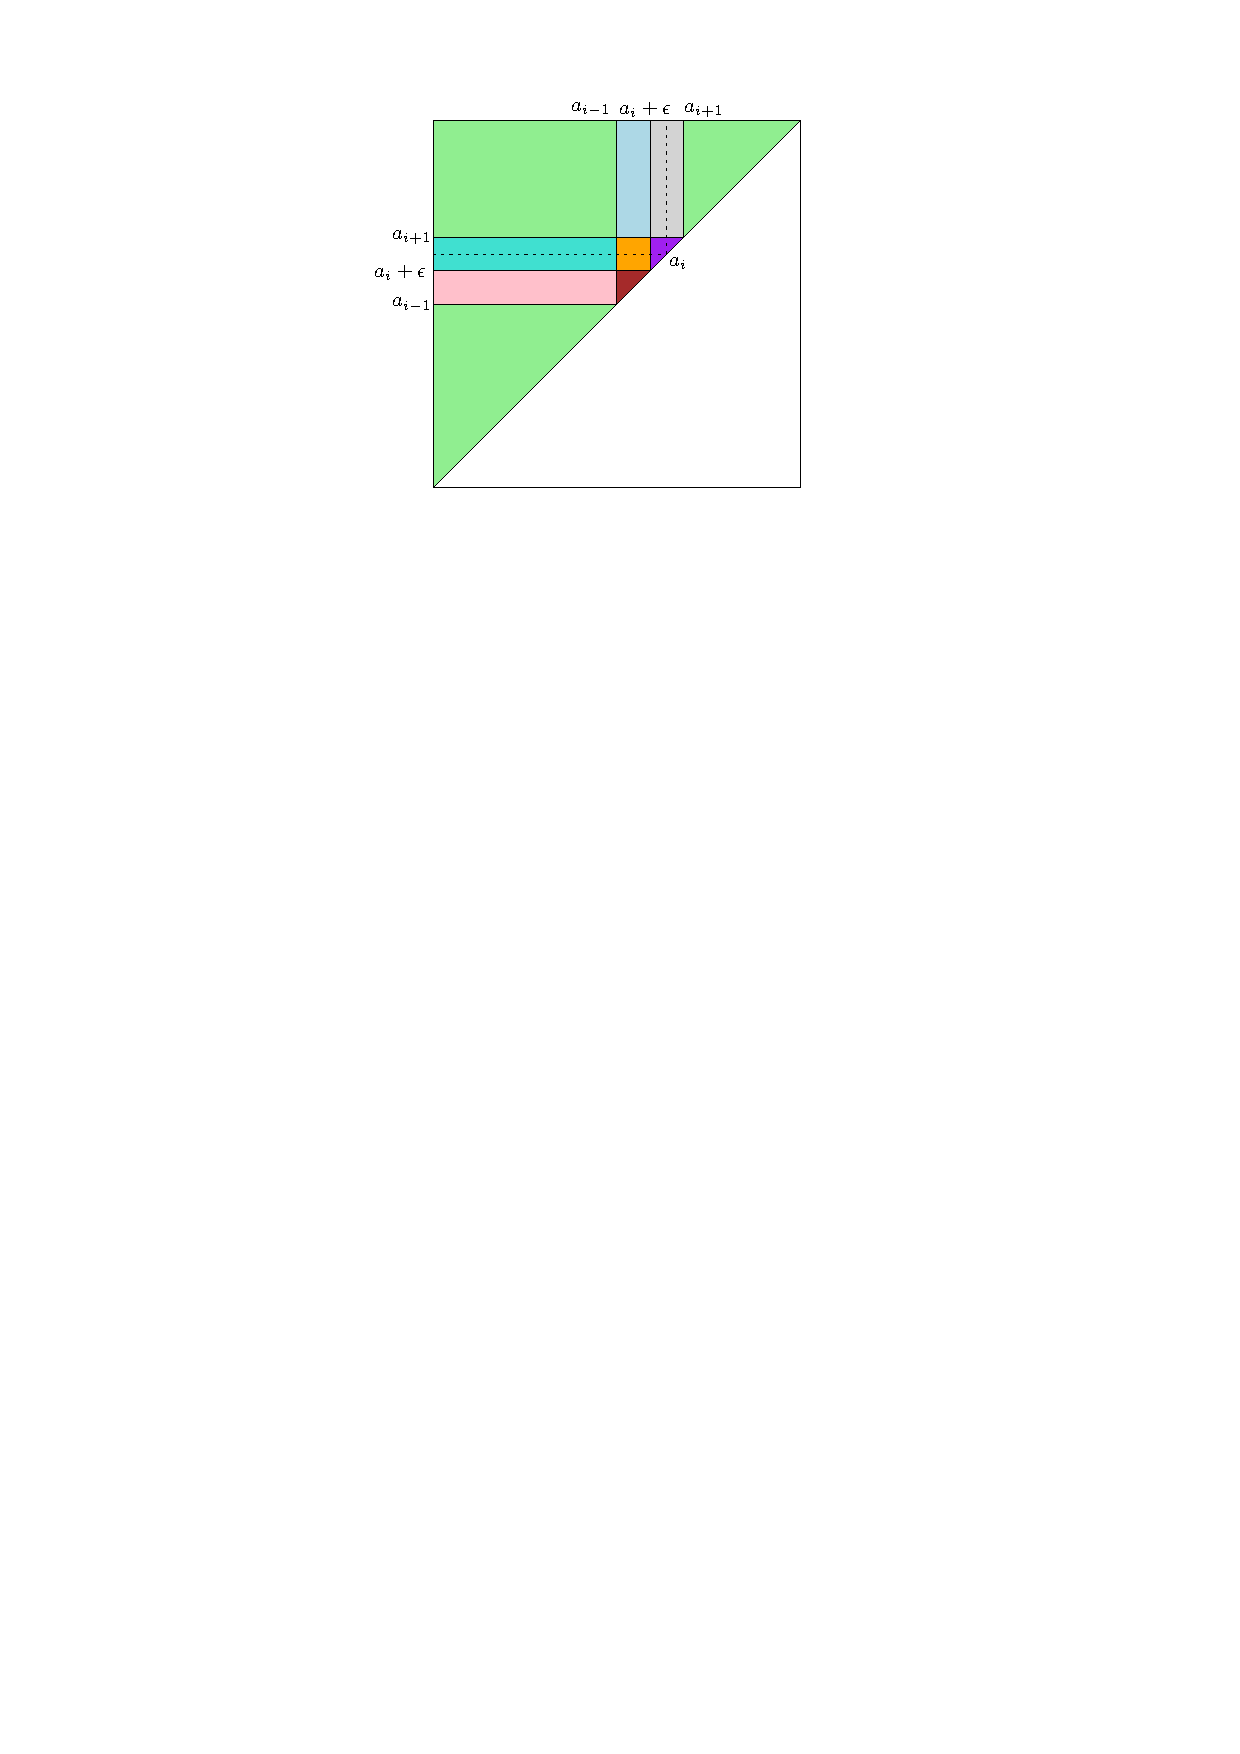
\includegraphics[width=7cm]{figures/ShiftAreas}
\caption[Persistence measure for Shift]{\label{fig:areashift}
%Left: Example of a Shift at $a_i$ with $\epsilon<0$.
%Right: 
Areas of the extended persistence diagram used in the proof, with $\e <0$.
}
\end{center}
\end{figure}

\end{proof}

%\section{Invariance Properties}
%\label{sec:invariance}
%In this section, given a telescope $T$, we characterize the evolution of $\Dg(\pi_2)$
%as we apply the operators of Section~\ref{sec:operator} to $T$.
%\subsection{Merge}
%\subsection{Split}
%\subsection{Shift}






































%%%%%%%%%%%%%%%%%%%%%%%%%%%%%%%%%%%%%%%%%%%%%%%%%%%%%%%%%%%%%%%%%%%%%%%%%%%
\section{A lower bound on $\distb$}
\label{sec:lowerbound}


In this section, we build on the Merge operator defined in the previous section and on the 
simplification operator defined in Section~\ref{sec:simplopReeb} to prove Theorem~\ref{th:locisom}.
Note that the upper bound in this theorem is given by Theorem~\ref{th:upperbound}
and always holds. The aim of this section is to prove the lower bound.

\paragraph*{Notation.} Henceforth, we write $\Reeb_f$ and $\Reeb_g$ instead of $\Reeb_f(X)$ and $\Reeb_g(Y)$ 
to avoid heavy notations. We also assume without loss of generality that $\max\{a_f,a_g\}=a_f$
and we let $\e=\distfd(\Reeb_f,\Reeb_g)$.

\paragraph*{Proof of Theorem~\ref{th:locisom}}
Let $K\in(0,1/22]$.
The proof proceeds by contradiction. Assuming that $\distb(\Reeb_f, \Reeb_g) < K\e$, 
where $\e=\distfd(\Reeb_f, \Reeb_g)< a_f/(8(1+22K))$, 
it  progressively transforms $\Reeb_g$ into some other Reeb graph $\Reeb_{g'}$ 
(Definition~\ref{def:simpl}) %in Section~\ref{sec:smoothope}) 
that satisfies both $\distfd(\Reeb_g, \Reeb_{g'})< 22K\e \leq \e$ (Proposition~\ref{prop:fdb}) %in Section~\ref{sec:Proof}) and   
and $\distfd(\Reeb_f, \Reeb_{g'})=0$ (Proposition~\ref{prop:iso2}). %in Section~\ref{sec:Proof}). 
The contradiction follows then from the triangle inequality. 

\subsection*{Graph Transformation}
\label{sec:smoothope}

The graph transformation is defined as the composition of the {\em Merge operator} from Section~\ref{sec:merge}
and the {\em simplification operator} from Section~\ref{sec:simplopReeb}. %\cite{Bauer14}. 
%We refer the reader to this article for the precise definitions. 
%Below we merely recall its main property.


%
\begin{defin}\label{def:simpl}
Let $\Reeb_f$ be a fixed Reeb graph with critical values $\{a_1,\cdots,a_n\}$. 
Given $\alpha > 0$, the full transformation $F_\alpha$ is defined as
%\begin{equation}\label{eq:fulltrans}
$$F_{\alpha}=\Merge_{9\alpha}\circ S_{2\alpha},$$
%\end{equation}
where $\Merge_{9\alpha}=\Merge_{a_n-9\alpha,\:a_n+9\alpha}\circ \cdots \circ \Merge_{a_1-9\alpha,\:a_1+9\alpha}$.
\end{defin}
See Figure~\ref{fig:recap3} for an illustration of this smoothing transformation.

\begin{figure}[htb]
\centering
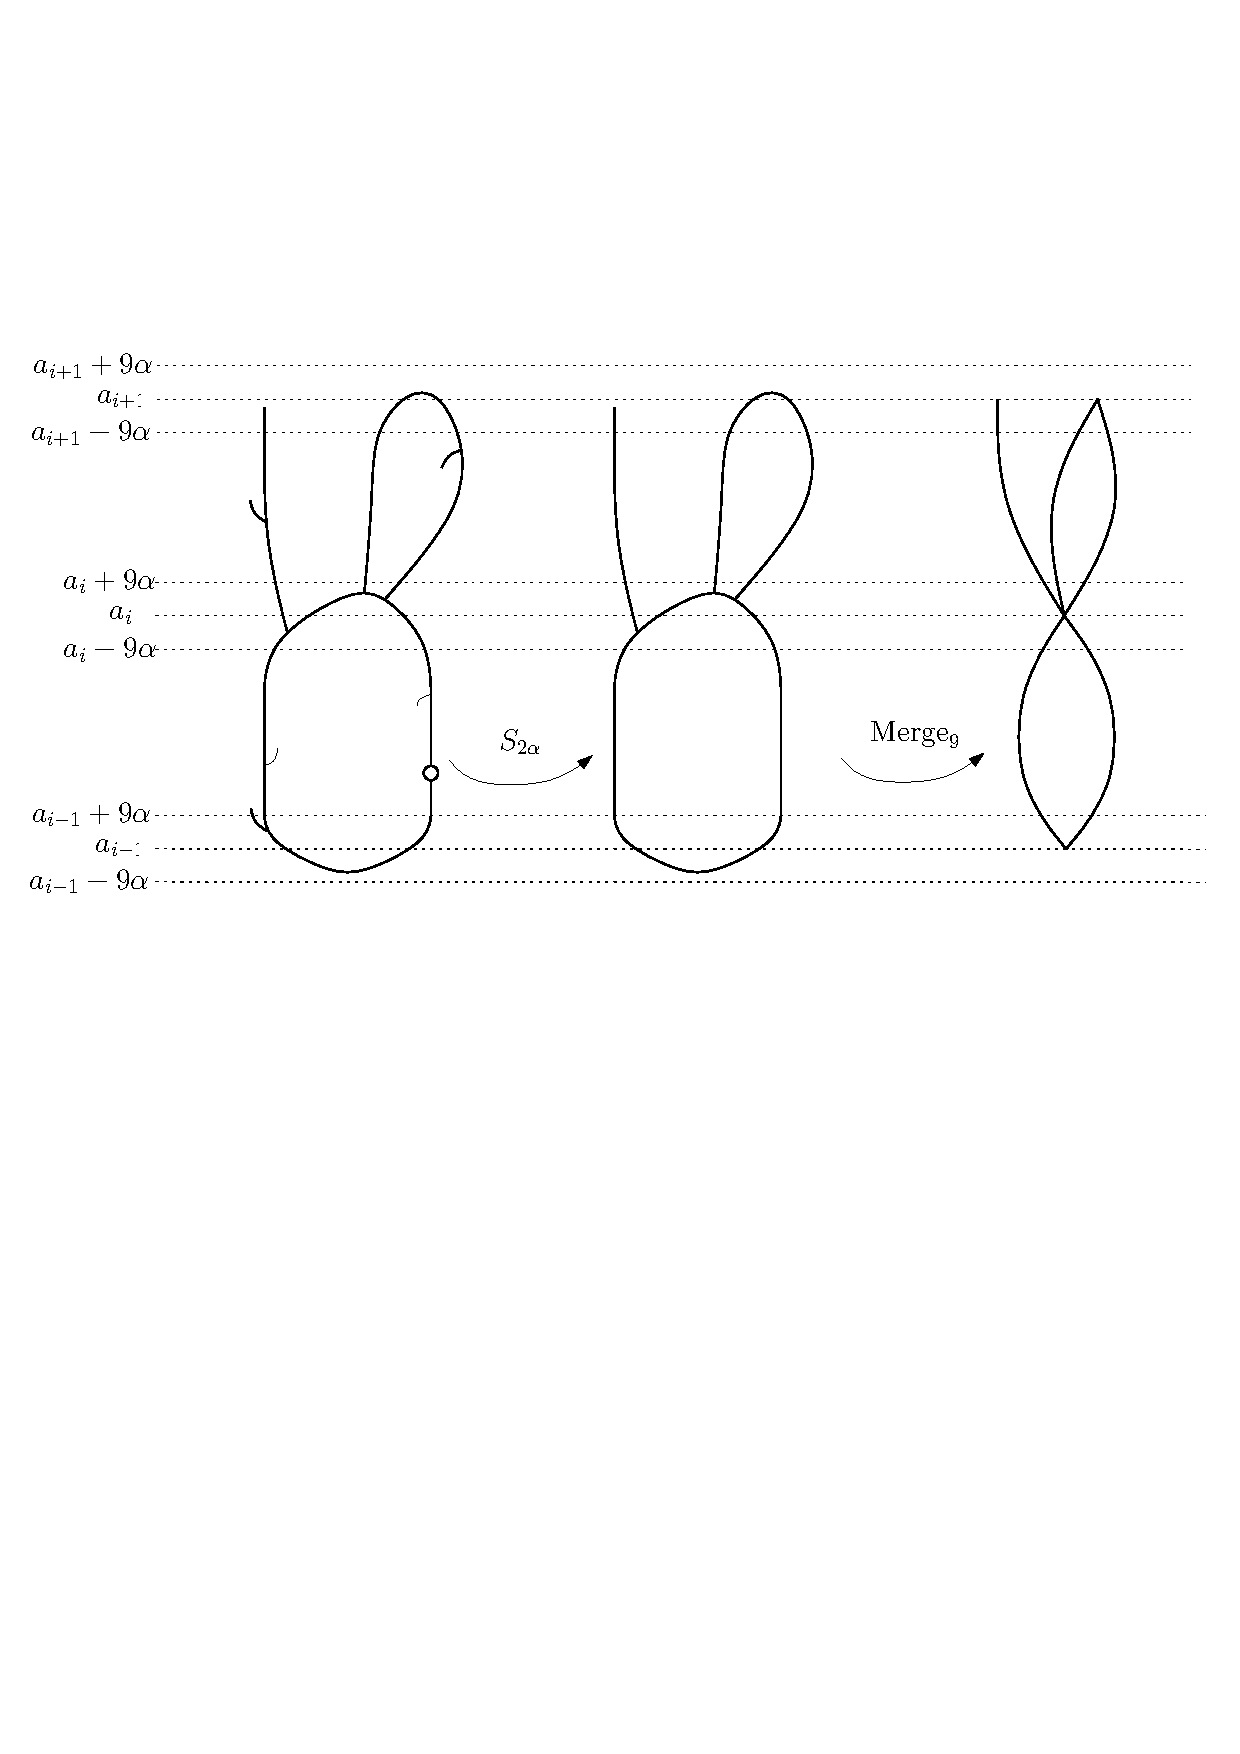
\includegraphics[width=11cm]{figures/FullTransform}
\caption[Simplification operator]{Illustration of $F_{\alpha}$ applied on an arbitrary Reeb graph.}
\label{fig:recap3}
\end{figure} 


\subsection*{Properties of the transformed graph}
\label{sec:Proof}

Let $\Reeb_f, \Reeb_g$ such that $\distb(\Reeb_f, \Reeb_g) < K\e$ 
where $\e=\distfd(\Reeb_f, \Reeb_g)< a_f/(8(1+22K))$.  Letting
$\Reeb_{g'} = F_{K\e}(\Reeb_g)$, we want to show both that
$\distfd(\Reeb_g,\Reeb_{g'})<22K\e\leq\e$ (Proposition~\ref{prop:fdb}) and $\distfd(\Reeb_f,\Reeb_{g'})=0$ (Proposition~\ref{prop:iso2}),
which will lead to a contradiction as mentioned previously.  
Let $B_\infty(x,r)$ denote the open ball of center $x$ and radius $r>0$ in the 
$\ell_\infty$-distance.

\begin{lem}\label{lem:crit}
Let $\Reeb_h=S_{2K\e}(\Reeb_g)$.
Under the above assumptions, one has 
\begin{equation}\label{eq:crit}
\Dg(h)\subset
{\bigcup}_{\tau\in\Dg(f)} B_\infty(\tau,9K\e).
%{\bigcup} \{B_\infty(\tau,9K\e):\tau\in\Dg(f)\}.
\end{equation}
\end{lem}

\begin{proof}
Let ${\rm off}_{K\e}(\Delta)=\{x\in\R^2\,:\,d_\infty(x,\Delta)\leq K\e\}$ be the $(K\e)$-offset
of the diagonal $\Delta$ in the $\ell_\infty$-distance.
Since $\distb(\Reeb_f,\Reeb_g)<K\e$, we have
$\Dg(g)\subset \bigcup_{\tau\in\Dg(f)} B_\infty(\tau,K\e) \cup {\rm off}_{K\e}(\Delta)$.
Since $\Reeb_h=S_{2K\e}(\Reeb_g)$,
%
it follows from Lemma~\ref{lem:stabsmooth} that $\distb(\Dg(h),\Dg(g))\leq 8K\e$.
Moreover, since every persistence pair in $\Dg(g)\cap{\rm off}_{K\e}(\Delta)$ is removed by $S_{2K\e}$,
it results that: 
$$\Dg(h)\subset{\bigcup}_{\tau\in\Dg(g)\setminus {\rm off}_{K\e}(\Delta)} B_\infty(\tau,8K\e)\subset{\bigcup}_{\tau\in\Dg(f)} B_\infty(\tau,9K\e).$$
\end{proof}

Now we can bound $\distfd(\Reeb_g,\Reeb_{g'})$. 
Recall that, given an arbitrary Reeb graph $\Reeb_h$, with critical values $\Crit(h)=\{c_1,...,c_p\}$,
if $C$ is a connected component of $h^{-1}(I)$, where $I$ is an open interval such that 
%$\exists c_i,c_{i+1}$ such that 
$I\subseteq(c_i,c_{i+1})$ for some $i$, 
then $C$ must be a {\em topological arc}, i.e. homeomorphic to an open interval.	

\begin{prop}\label{prop:fdb}
Under the same assumptions as above,  
one has $\distfd(\Reeb_g,\Reeb_{g'})<22K\epsilon$.
\end{prop}

\begin{figure}\centering
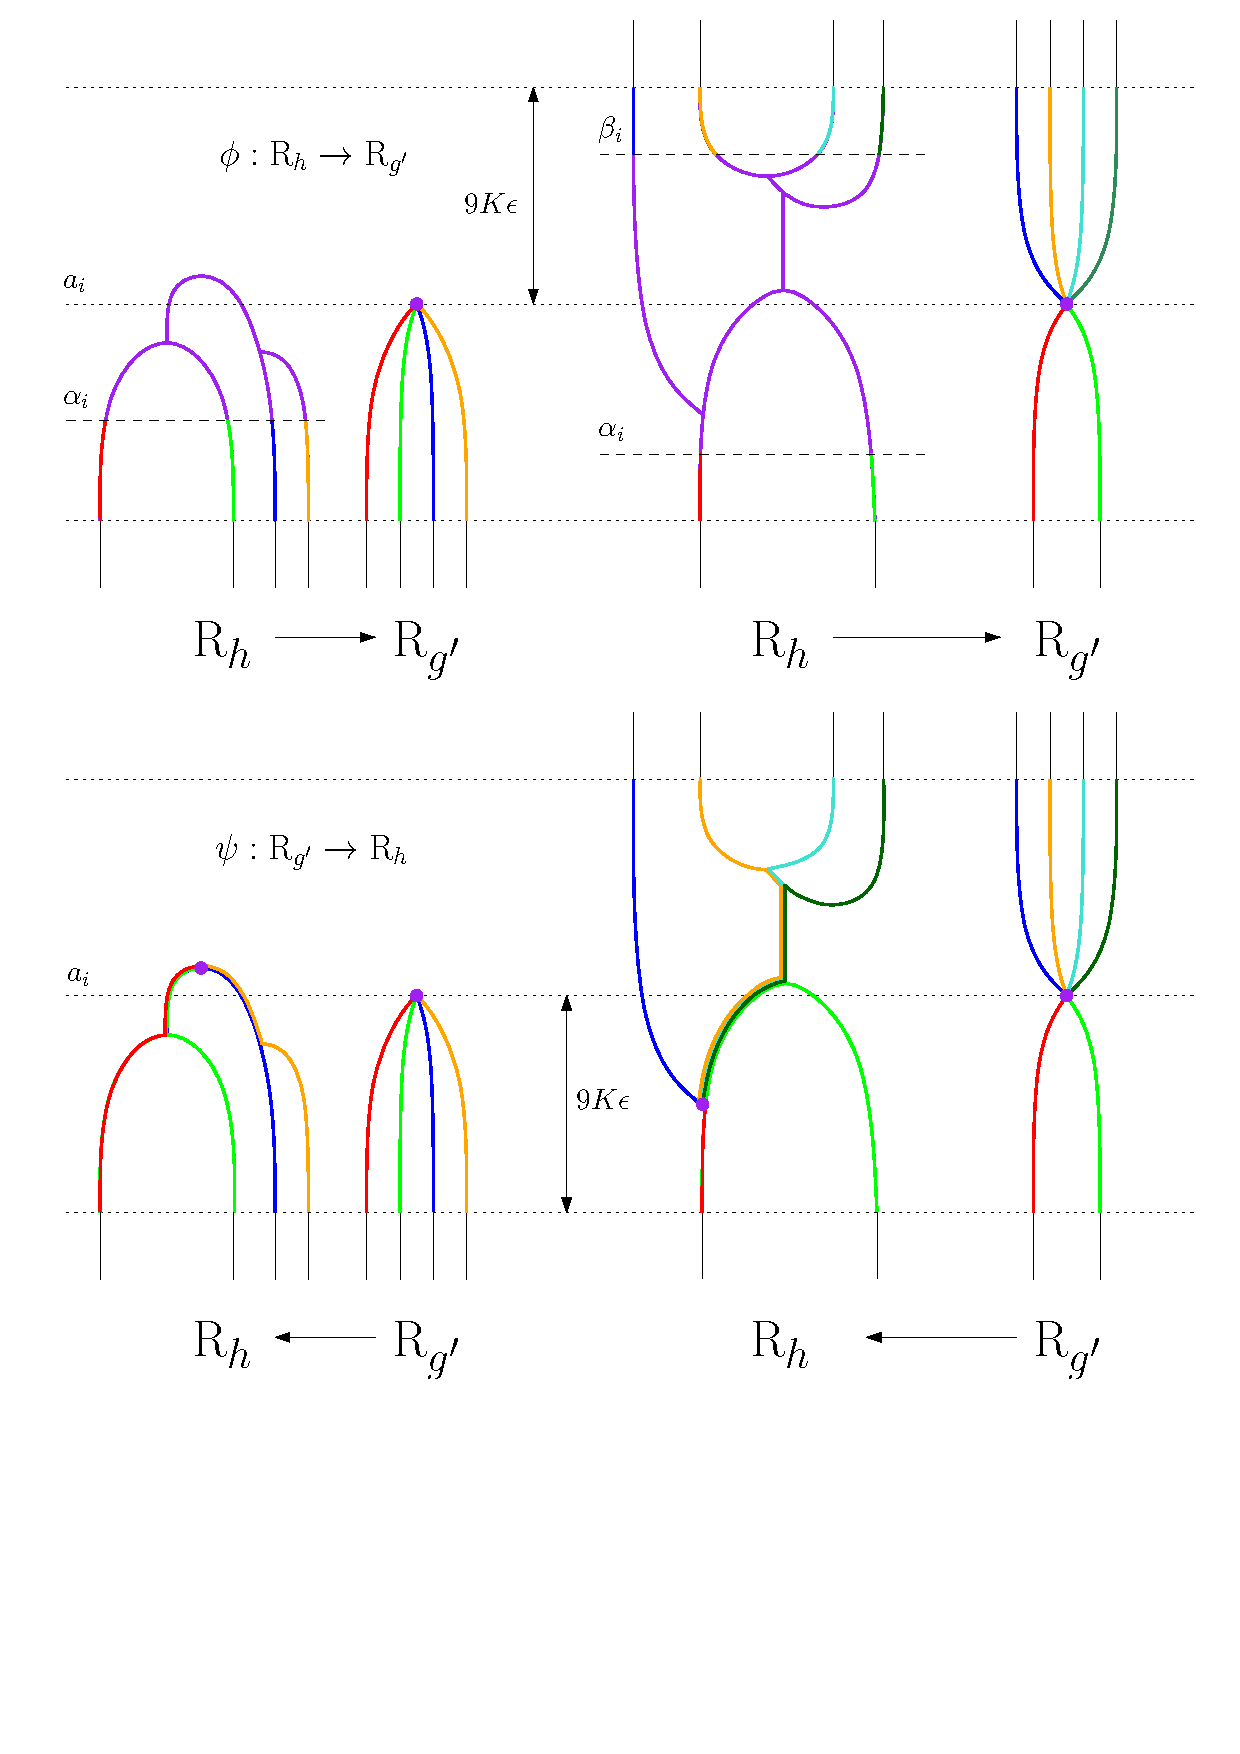
\includegraphics[width=14cm]{figures/ContinuousMaps}
\caption[Continuous maps]{\label{fig:fdmerge}
The effects of $\phi$ and $\psi$ around a specific critical value $a_i$ of $f$. Segments are matched according
to their colors (up to reparameterization).
}
\end{figure}

\begin{proof}
Let $\Reeb_h=S_{2K\e}(\Reeb_g)$.
The triangle inequality asserts that 
\[
\distfd(\Reeb_{g'},\Reeb_g)\leq \distfd(\Reeb_{g'},\Reeb_h)+\distfd(\Reeb_h,\Reeb_g).
\]
It suffices therefore to bound both
$\distfd(\Reeb_{g'},\Reeb_h)$ and $\distfd(\Reeb_h,\Reeb_{g})$.
By Lemma~\ref{lem:stabsmooth}, we have $\distfd(\Reeb_h,\Reeb_g) < 4K\e$.
Now, recall from~(\ref{eq:crit}) that the points of the extended
persistence diagram of $\Reeb_h$ are included in
${\bigcup}_{\tau\in\Dg(f)} B_\infty(\tau,9K\e)$.  Moreover, since
$\Reeb_{g'}=\Merge_{9K\e}(\Reeb_h)$, $\Reeb_{g'}$ and $\Reeb_h$ are
composed of the same number of arcs in each $[a_i+9K\e,a_{i+1}-9K\e]$.
Hence, we can define explicit continuous maps
$\phi:\Reeb_h\rightarrow\Reeb_{g'}$ and
$\psi:\Reeb_{g'}\rightarrow\Reeb_h$ as depicted in
Figure~\ref{fig:fdmerge}.  More precisely, since $\Reeb_h$ and
$\Reeb_{g'}$ are composed of the same number of arcs in each
$[a_i+9K\e,a_{i+1}-9K\e]$, we only need to specify $\phi$ and $\psi$
inside each interval $(a_i-9K\e,a_i+9K\e)$.  Since the critical values
of $\Reeb_h$ are within distance less that $9K\e$ of the critical
values of $f$, there exist two levels $a_i-9K\e < \alpha_i\leq\beta_i
< a_i+9K\e$ such that $\Reeb_h$ is only composed of arcs in
$(a_i-9K\e,\alpha_i]$ and $[\beta_i,a_i+9K\e)$ for each $i$ (dashed
    lines in Figure~\ref{fig:fdmerge}).  For any connected component~$C$ of
    $h^{-1}((a_i-9K\e,a_i+9K\e))$, the map $\phi$ sends all points of
    $C\cap h^{-1}([\alpha_i,\beta_i])$ to the corresponding critical
    point $y_C$ created by the Merge in $\Reeb_{g'}$, and it maps the
    arcs of $C\cap h^{-1}((a_i-9K\e,\alpha_i])$ and $C\cap
    h^{-1}([\beta_i,a_i+9K\e))$ to the corresponding arcs in
    $\Reeb_{g'}$.  In return, the map $\psi$ sends the critical
    point~$y_C$ to an arbitrary point of $C$.  Then, since the Merge
    operation preserves connected components, for each arc $A'$ of
    $(g')^{-1}((a_i-9K\e,a_i+9K\e))$ connected to~$y_C$, there is at
    least one corresponding path $A$ in $\Reeb_h$ whose endpoint in
    $h^{-1}(a_i-9K\e)$ or $h^{-1}(a_i+9K\e)$ matches with the one of $A'$
    (see the colors in the second row of Figure~\ref{fig:fdmerge}).  Hence $\psi$ sends
    $A'$ to $A$.

\noindent Let us bound the
three terms in the $\max\{\cdots\}$ in~(\ref{eq:dfd})
with this choice of maps $\phi, \psi$: 
\begin{itemize}
\item We first  bound $\|h-g'\circ\phi\|_\infty$. Let $x\in\Reeb_h$. Either $h(x)\in \bigcup_{i\in\{1,...,n-1\}} [a_i+9K\e,a_{i+1}-9K\e]$,  
and in this case we have $h(x)=g'(\phi(x))$ by definition of~$\phi$;
or, there is $i_0\in\{1,...,n\}$ such that $h(x)\in (a_{i_0}-9K\e,a_{i_0}+9K\e)$ and then $g'(\phi(x))\in (a_{i_0}-9K\e,a_{i_0}+9K\e)$.
In both cases $|h(x)-g'\circ\phi(x)| < 18K\e$. Hence, $\|h-g'\circ\phi\|_\infty < 18K\e$.
\item Since the previous proof is symmetric in $h$ and $g'$, one also has $\|g'-h\circ\psi\|_\infty < 18K\e$.
\item We now bound $D(\phi,\psi)$. Let $(x,\phi(x)),(\psi(y),y)\in C(\phi,\psi)$ (the cases $(x,\phi(x)),(x',\phi(x'))$
and $(\psi(y),y),(\psi(y'),y')$ are similar). Let $\pi_{g'}:[0,1]\rightarrow\Reeb_{g'}$ be a continuous path from $\phi(x)$ to $y$  
which achieves $d_{g'}(\phi(x),y)$.
\begin{itemize}
\item Assume $h(x)\in \bigcup_{i\in\{1,...,n-1\}} [a_i+9K\e,a_{i+1}-9K\e]$. Then one has $\psi\circ\phi(x)=x$.
Hence, $\pi_h=\psi\circ\pi_{g'}$ is a valid path from $x$ to $\psi(y)$. Moreover, since $\|g'-h\circ\psi\|_\infty < 18K\e$,
it follows that
\begin{equation}\label{eqs:noname}
\begin{array}{l}\max\ \im(h\circ \pi_{h}) < \max\ \im(g'\circ \pi_{g'}) +18K\e,\\[0.5ex]
\min\ \im(h\circ\pi_{h}) > \min\ \im(g'\circ\pi_{g'}) -18K\e.\end{array}
\end{equation}
Hence, one has 
$$\begin{array}{l}d_h(x,\psi(y))\leq \max\ \im(h\circ\pi_{h})-\min\ \im(h\circ\pi_{h}) < d_{g'}(\phi(x),y)+36K\e,\\
-d_h(x,\psi(y))\geq \min\ \im(h\circ\pi_{h})-\max\ \im(h\circ\pi_{h}) > -d_{g'}(\phi(x),y)-36K\e.\end{array}$$
This shows that $|d_h(x,\psi(y))-d_{g'}(\phi(x),y)| < 36K\e$.
\item Assume that there is $i_0\in\{1,...,n\}$ such that $h(x)\in(a_{i_0}-9K\e,a_{i_0}+9K\e)$.
Then, by definition of $\phi, \psi$, we have  $g'(\phi(x))\in(a_{i_0}-9K\e,a_{i_0}+9K\e)$, and
there is a path
$\pi'_{h}:[0,1]\rightarrow\Reeb_h$ from $x$ to $\psi\circ\phi(x)$
within the interval $(a_{i_0}-9K\e,a_{i_0}+9K\e)$, which itself is
included in the interior of the offset ${\rm off}_{18K\e}({\rm im}(g'\circ\pi_{g'}))$. Let now
$\pi_h$ be the concatenation of $\pi'_h$ with $\psi\circ\pi_{g'}$, which goes from $x$ to
$\psi(y)$.
Since $\|g'-h\circ\psi\|<18K\e$, it follows that 
${\rm im}(h\circ\psi\circ\pi_{g'})\subseteq {\rm int}\ {\rm off}_{18K\e}({\rm im}(g'\circ\pi_{g'}))$, and since 
${\rm im}(h\circ\pi_h)={\rm im}(h\circ\pi'_h)\cup{\rm im}(h\circ\psi\circ\pi_{g'})$ by
concatenation, one finally has $${\rm im}(h\circ\pi_h)\subseteq {\rm
  int}\ {\rm off}_{18K\e}({\rm im}(g'\circ\pi_{g'})).$$ Hence, the 
inequalities of~(\ref{eqs:noname}) hold, implying that $|d_h(x,\psi(y))-d_{g'}(\phi(x),y)| < 36K\e$.
\end{itemize} 
Since these inequalities hold for any $(x,\phi(x))$ and $(\psi(y),y)$, we deduce that $D(\phi,\psi) \leq 36K\e$.
\end{itemize}
Thus,
$\distfd(\Reeb_{h},\Reeb_g)<4K\e$  and $\distfd(\Reeb_h,\Reeb_{g'})\leq 18K\e$, so
$\distfd(\Reeb_{g'},\Reeb_g) < 22K\e$ as desired.
\end{proof}

To complete the proof, we now show that $\Reeb_{g'}$ is isomorphic to $\Reeb_f$. %(i.e. it lies at functional distortion distance~$0$).  

\begin{prop}\label{prop:iso2}
Under the same assumptions as above,  
one has $\distfd(\Reeb_f,\Reeb_{g'})=0$.
\end{prop}

\begin{proof}
First, recall from~(\ref{eq:crit}) that the points of the extended
persistence diagram of $\Reeb_h$ are included in
${\bigcup}_{\tau\in\Dg(f)} B_\infty(\tau,9K\e)$.
Since $\Reeb_{g'}=\Merge_{9K\e}(\Reeb_h)$, 
it follows from Lemma~\ref{lem:mergeprop} that $\Crit(g')\subseteq\Crit(f)$.
Hence, both $\Reeb_{g'}$ and $\Reeb_f$ are composed of arcs in each $(a_i,a_{i+1})$.

Now, we show that, for each $i$, the number of arcs of $(g')^{-1}((a_i,a_{i+1}))$
and $f^{-1}((a_i,a_{i+1}))$ are the same.
By the triangle inequality and Proposition~\ref{prop:fdb}, we have: 
\begin{equation}\label{eq:tri}
\distfd(\Reeb_f,\Reeb_{g'}) \leq  \distfd(\Reeb_f,\Reeb_g)  + \distfd(\Reeb_g,\Reeb_{g'}) < (1+22K)\e.
\end{equation}
Let $\phi:\Reeb_f\rightarrow\Reeb_{g'}$ and $\psi:\Reeb_{g'}\rightarrow\Reeb_f$
be optimal continuous maps that achieve $\distfd(\Reeb_f,\Reeb_{g'})$.
Let $i\in\{1,...,n-1\}$.
Assume that there are more arcs of $f^{-1}((a_i,a_{i+1}))$ 
than arcs of $(g')^{-1}((a_i,a_{i+1}))$. For every arc $A$ of
$f^{-1}((a_i,a_{i+1}))$, let $x_A\in A$ such that $f(x_A)=\bar{a}=\frac{1}{2}(a_i+a_{i+1})$.
%
First, note that $\phi(x_A)$ must belong to an arc of 
$(g')^{-1}((a_i,a_{i+1}))$. Indeed, since $\|f-g'\circ\phi\|_\infty < (1+22K\e)$,
one has $g'(\phi(x_A))\in(\bar{a}-(1+22K)\e,\bar{a}+(1+22K)\e)\subseteq(a_i,a_{i+1})$.
%
Then, according to the pigeonhole principle,
there exist $x_A,x_{A'}$ such that $\phi(x_A)$ and $\phi(x_{A'})$
belong to the same arc of $(g')^{-1}((a_i,a_{i+1}))$.
%
\begin{itemize}
\item Since $x_A$ and $x_{A'}$ do not belong to the same arc, we have
$$d_f(x_{A},x_{A'}) > a_f/2.$$

\item Now, since $\|f-g'\circ\phi\|_\infty<(1+22K)\e$ and $\phi(x_{A}),\phi(x_{A'})$ belong to the same arc of $(g')^{-1}((a_i,a_{i+1}))$,
we also have (see Figure~\ref{fig:smallBranches} for an illustration):
$$d_{g'}(\phi(x_{A}),\phi(x_{A'})) < 2(1+22K)\e.$$
\end{itemize}
%
\begin{figure}[h]\centering
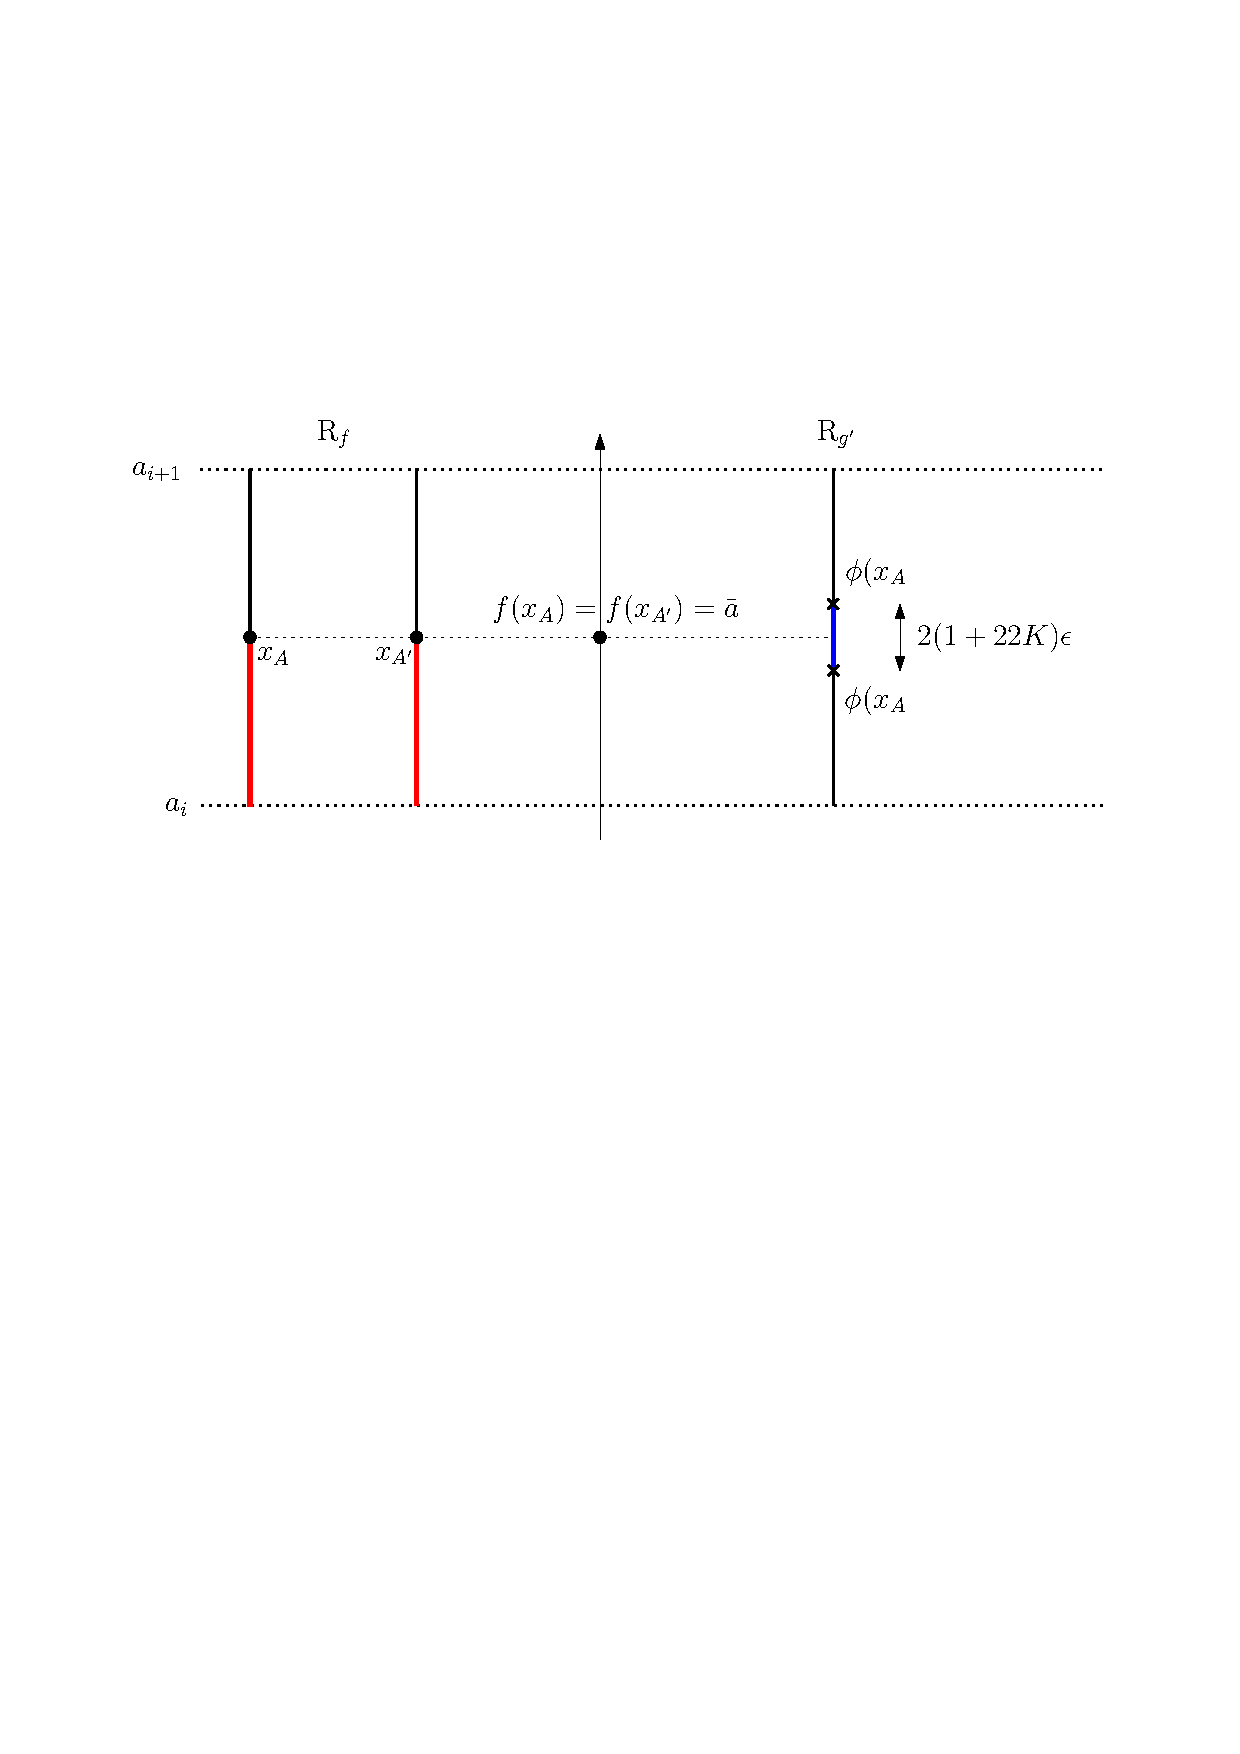
\includegraphics[width=10cm]{figures/Arcs}
\caption[Arc number argument]{\label{fig:smallBranches} Any path between $x_A$ and $x_{A'}$ must contain the red segments, and the blue segment is a
particular path between $\phi(x_A)$ and $\phi(x_{A'})$.}
\end{figure}



Hence, $D(\phi, \psi) \geq
|d_f(x_A,x_{A'})-d_{g'}(\phi(x_{A}),\phi(x_{A'}))|> a_f/2-2(1+22K)\e$,
which is greater than $2(1+22K)\e$ because $\e<a_f/(8(1+22K))$. Thus,
$\distfd(\Reeb_f,\Reeb_{g'})>(1+22K)\e$, which leads to a
contradiction with~(\ref{eq:tri}).  This means that there cannot be
more arcs in $f^{-1}((a_i,a_{i+1}))$ than in $(g')^{-1}((a_i,a_{i+1}))$.
Since the proof is symmetric in $f$ and $g'$, the numbers of arcs in
$(g')^{-1}((a_i,a_{i+1}))$ and in $f^{-1}((a_i,a_{i+1}))$ are actually the
same.

Finally, we show that the attaching maps of these arcs are also the
same.  In this particular graph setting, this is equivalent to showing
that corresponding arcs in $\Reeb_f$ and $\Reeb_{g'}$ have the same
endpoints.  Let $a_i$ be a critical value. Let $A_{f,i}^-$ and
$A_{f,i}^+$ (resp. $A_{g',i}^-$ and $A_{g',i}^+$) be the sets of arcs
in $f^{-1}((a_{i-1},a_i))$ and $f^{-1}((a_{i},a_{i+1}))$
(resp. $(g')^{-1}((a_{i-1},a_i))$ and $(g')^{-1}((a_{i},a_{i+1}))$).
Morevover, we let $\zeta_f^i$ and $\xi_f^i$ (resp. $\zeta_{g'}^i$ and
$\xi_{g'}^i$) be the corresponding attaching maps that send arcs to
their endpoints in $f^{-1}(a_i)$ (resp. $(g')^{-1}(a_i)$).  Let
$A,B\in A_{f,i}^-$. We define an equivalence relation $\sim_{f,i}$
between $A$ and $B$ by: $A\sim_{f,i} B$ if and only if $\zeta_f^i(A)=\zeta_f^i(B)$,
i.e. the endpoints of the arcs in the critical slice $f^{-1}(a_i)$ are
the same.  Similarly, $C,D\in A_{f,i}^+$ are equivalent if and only if
$\xi_f^i(C)=\xi_f^i(D)$.  One can define $\sim_{g',i}$ in the same way.
%
To show that the attaching maps of $\Reeb_f$ and $\Reeb_{g'}$ are the same,
we need to find a bijection $b$ between the arcs of $\Reeb_f$ and $\Reeb_{g'}$ 
such that $A\sim_{f,i}B \Leftrightarrow b(A)\sim_{g',i}b(B)$ for each $i$.

We will now define $b$ then check that it satisfies the condition.
Recall from~(\ref{eq:tri}) that 
$\distfd(\Reeb_f,\Reeb_{g'})< (1+22K)\e.$
Hence there exists a continuous map $\phi:\Reeb_f\rightarrow\Reeb_{g'}$ such that
$\|f-g'\circ\phi\|_\infty < (1+22K)\e$.
This map induces a bijection $b$ between the arcs of $\Reeb_f$ and $\Reeb_{g'}$.
Indeed, given an arc $A\in A_{f,i}^-$, let $x\in A$ such that $f(x)=\bar{a}=\frac{1}{2}(a_{i-1}+a_i)$. 
We define $b(A)$ as the arc of $A_{g,i}^-$ that contains $\phi(x)$.
The map $b$ is well-defined since 
$g'\circ\phi(x)\in\left[\bar a-(1+22K)\e,\bar a+(1+22K)\e\right]\subseteq(a_{i-1},a_i),$
hence $\phi(x)$	must belong to an arc of $(g')^{-1}((a_{i-1},a_i))$.
Let us show that  $b(A)\sim_{g',i}b(B)\Rightarrow A\sim_{f,i} B$.
Assume there exist $A,B\in A_{f,i}^-$ (the treatment of $A,B\in A_{f,i}^+$ is similar) such that $A\not\sim_{f,i} B$
and $b(A)\sim_{g',i} b(B)$. 
Let $x=\zeta_f^i(A)$ and $y=\zeta_f^i(B)$. Then we have $d_f(x,y)\geq a_f$ while $d_{g'}(\phi(x),\phi(y)) < 2(1+22K)\e$
(see Figure~\ref{fig:attach}).
Hence $|d_f(x,y)-d_{g'}(\phi(x),\phi(y))| > a_f - 2(1+22K)\e > 2(1+22K)\e$,
so $\distfd(\Reeb_f,\Reeb_{g'}) > (1+22K)\e$, which leads to a contradiction with~(\ref{eq:tri}).
The same argument applies to show that $ A\sim_{f,i} B\Rightarrow b(A)\sim_{g',i}b(B)$.
\end{proof}

\begin{figure}[h]\centering
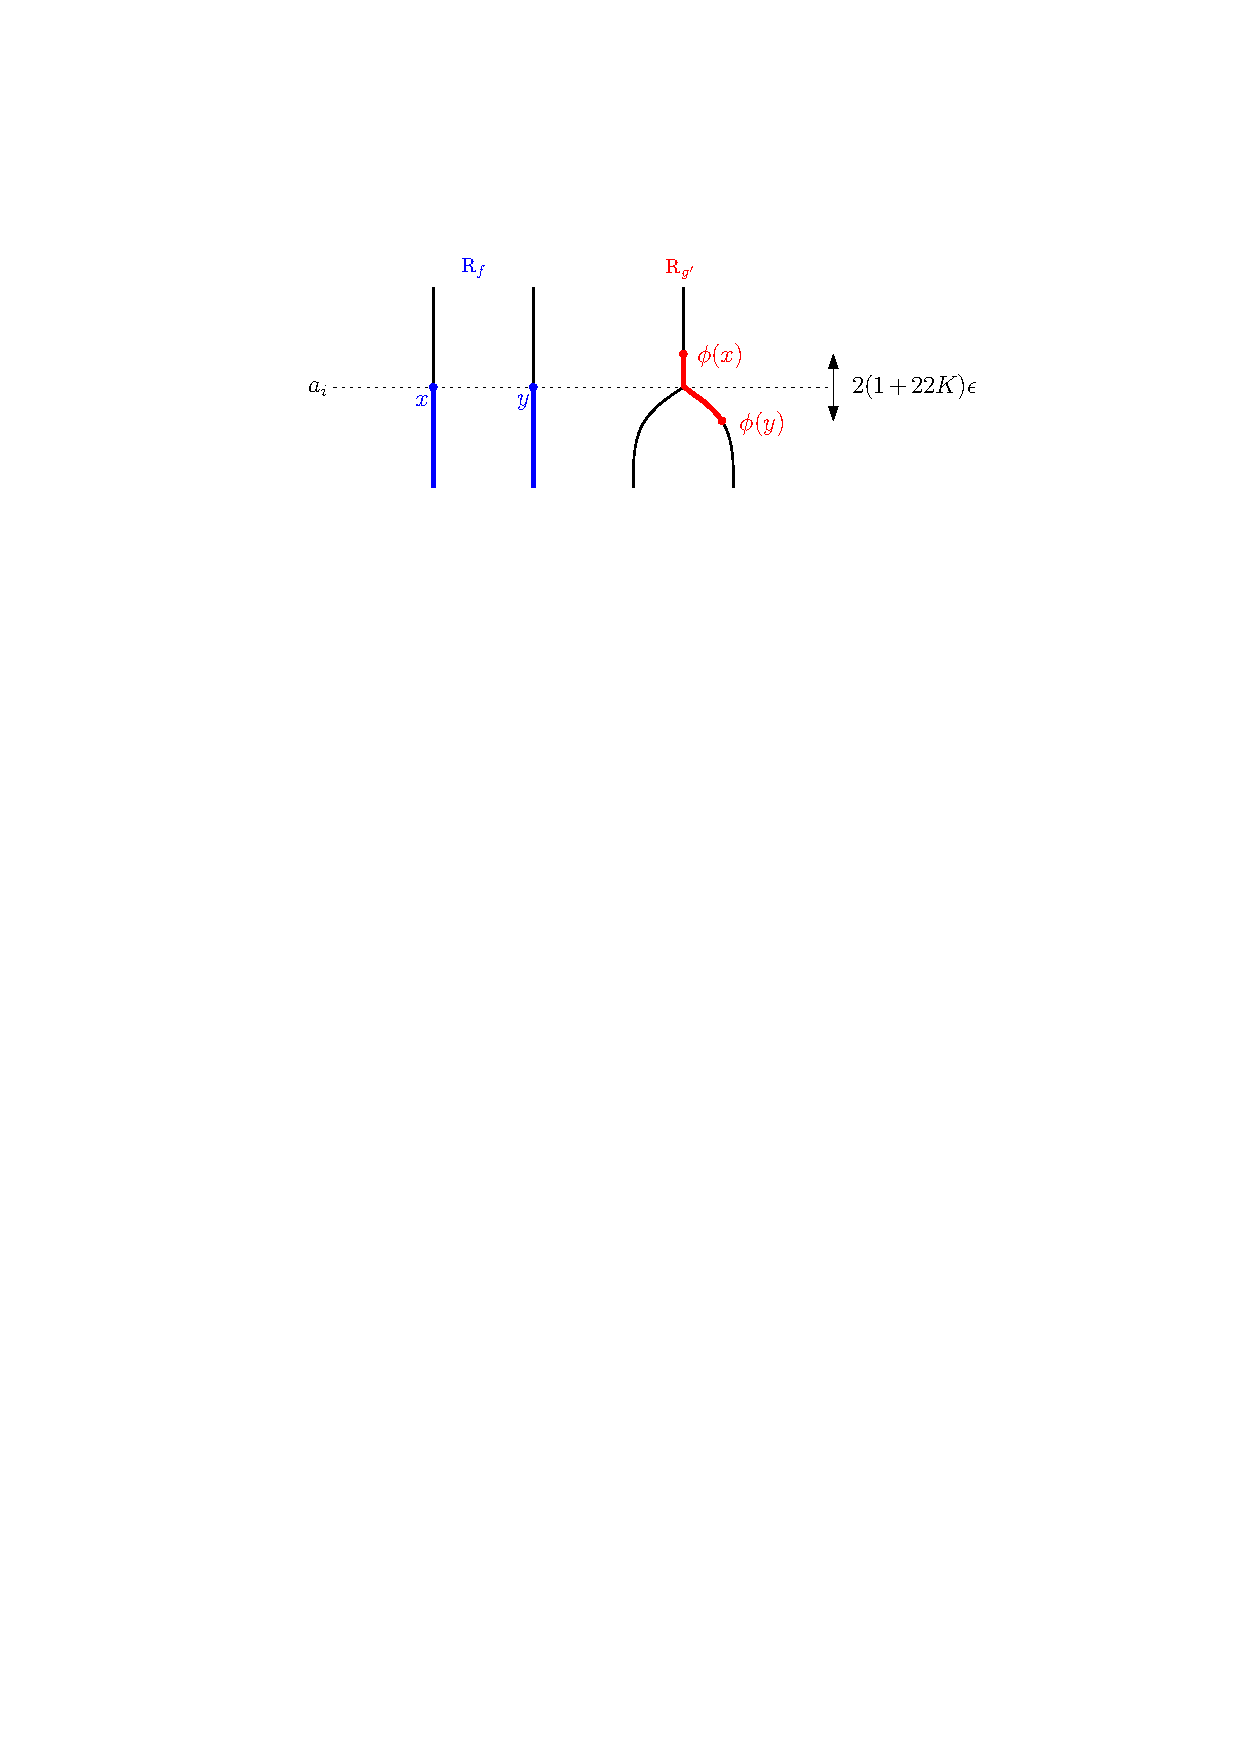
\includegraphics[width=7.5cm]{figures/AttachingMaps}
\caption[Branching argument]{Any path from $x$ to $y$ must go through an entire arc, hence $d_f(x,y)\geq a_f$.
On the contrary, there exists a direct path (displayed in red) between $\phi(x)$ and $\phi(y)$, hence $d_{g'}(\phi(x),\phi(y)) < 2(1+22K)\e$.}
\label{fig:attach}
\end{figure}

Hence, $\distb$ and $\distfd$ are locally equivalent, and so are $\distb$ and $\distfgh$ thanks to Theorem~\ref{th:dfddfgheq}.
%In particular, it follows that their {\em induced intrinsic metrics} $\hdistb$ and $\hdistfd$ are {\em globally} equivalent.




















%%%%%%%%%%%%%%%%%%%%%%%%%%%%%%%%%%%%%%%%%%%%%%%%%%%%%%%%%%%%%%%%%%%%%%%%%%%
\section{Induced Metrics}
\label{sec:induced}

%\paragraph*{Intrinsic metrics.}
A desired property for dissimilarity measures is to be {\em intrinsic}, i.e. realized as the lengths of shortest continuous 
paths in the space of Reeb graphs~\cite{Burago01}. This is particularly useful when one actually needs to interpolate between data, 
and not just discriminate between them, which happens in applications such as 
image or 3D shape morphing, skeletonization, and matching~\cite{Ge11, Mohamed12, Mukasa06, Tierny06}. 
Unfortunately, all the  metrics proposed so far for Reeb graphs fail according to this criterion.   
Defining intrinsic metrics would not only open the door to the use of Reeb graphs in the aforementioned applications, 
but it would also provide a better understanding of the intrinsic structure of the space of Reeb graphs, and give a deeper meaning to the distance values.

In this section, we leverage the local equivalence given by
Theorem~\ref{th:locisom} to derive a global equivalence between
the intrinsic metrics $\hdistb$ and $\hdistfd$ induced by $\distb$ and
$\distfd$.  Note that we already know $\hdistfd$ to be equivalent to
$\hdistfgh$ %and $\hdisti$ 
since $\distfd$ is equivalent
to $\distfgh$. %and $\disti$.

\paragraph*{Notation.} 
Let $\RS$ denote the space of Reeb graphs coming from Morse-type functions.
In the following, whatever the metric  
$d:\RS\times\RS\rightarrow\R_+$ under consideration, we define the 
class of {\em admissible paths} in
$\RS$ to be those maps $\gamma:[0,1]\rightarrow\RS$ that are
continuous in $\distfd$. This makes sense when $d$ is either $\distfd$
itself or $\distfgh$, %or $\disti$, all of 
which is equivalent to $\distfd$ and therefore admits the same continuous maps
$\gamma:[0,1]\rightarrow\RS$. In the case $d=\distb$ our convention
means restricting the class of admissible paths to a strict subset of
the maps $\gamma:[0,1]\rightarrow\RS$ that are continuous in~$\distb$ (by
Theorem~\ref{th:upperbound}), which is required by some of our
following claims.

\begin{defin}
Let $d:\RS\times\RS\rightarrow\R_+$ be a metric on $\RS$. Let $\Reeb_f,\Reeb_g\in\RS$,
and $\gamma:[0,1]\rightarrow\RS$ be an admissible path such that $\gamma(0)=\Reeb_f$ and $\gamma(1)=\Reeb_g$.
The {\em length} of $\gamma$ induced by $d$ is defined as
$L_d(\gamma)= \sup_{n,\Sigma}\ \sum_{i=0}^{n-1} d(\gamma(t_{i}), \gamma(t_{i+1}))$
where $n$ ranges over~$\N$ and $\Sigma$ ranges over all partitions $0=t_0\leq t_1\leq ... \leq t_n=1$ of $[0,1]$.
%
The {\em intrinsic metric induced by $d$}, denoted $\hat d$, is defined by
%
$\hat d(\Reeb_f,\Reeb_g)=\rm{inf}_\gamma\ L_d(\gamma)$
%
where $\gamma$ ranges over all admissible paths $\gamma:[0,1]\rightarrow\RS$ 
such that $\gamma(0)=\Reeb_f$ and $\gamma(1)=\Reeb_g$.
\end{defin}

\paragraph*{Strong equivalence of induced metrics.} The following result is, in our view, the starting point for the study
of intrinsic metrics over the space of Reeb graphs. It comes as a
consequence of the (local or global) equivalences between $\distb$ and
$\distfd$ stated in Theorems~\ref{th:upperbound} and~\ref{th:locisom}.
The intuition is that integrating two locally equivalent metrics along
the same path using sufficiently small integration steps
yields the same total length up to a constant factor, hence the
global equivalence between the induced intrinsic
metrics\footnote{Provided the induced metrics are defined using the
  same class of admissible paths, hence our convention.}.


\begin{thm}\label{th:strongeq}
$\hdistb$ and $\hdistfd$ are globally equivalent. Specifically, for any $\Reeb_f,\Reeb_g\in\RS$,
\begin{equation}\label{eq:strongeq}
\hdistfd(\Reeb_f,\Reeb_g)/\const\leq \hdistb(\Reeb_f,\Reeb_g)\leq 2\,\hdistfd(\Reeb_f,\Reeb_g).
\end{equation}
\end{thm}


\begin{proof}
We first show that $\hdistb(\Reeb_f,\Reeb_g)\leq 2\,\hdistfd(\Reeb_f,\Reeb_g)$. 
Let $\gamma$ be an admissible path 
and let $\Sigma=\{t_0,...,t_n\}$ be a partition of $[0,1]$.
Then, by Theorem~\ref{th:upperbound}, 
$$\sum_{i=0}^{n-1} \distfd(\gamma(t_{i}), \gamma(t_{i+1}))\geq
\frac{1}{2}\sum_{i=0}^{n-1} \distb(\gamma(t_{i}), \gamma(t_{i+1})).$$
Since this is true for any partition $\Sigma$ of any finite size $n$, it
follows that
$$L_{\distfd} (\gamma) \geq \frac{1}{2} L_{\distb}(\gamma)\geq\frac{1}{2} \hdistb(\Reeb_f,\Reeb_g).$$
Again, this inequality holds for any admissible path $\gamma$, so $\hdistb(\Reeb_f,\Reeb_g)\leq 2\hdistfd(\Reeb_f,\Reeb_g)$. \\
%
We now show that $\hdistfd(\Reeb_f,\Reeb_g)/\const\leq \hdistb(\Reeb_f,\Reeb_g)$.
Let $\gamma$ be an admissible path 
and $\Sigma=\{t_0,...,t_n\}$ a partition of $[0,1]$.  We claim that
there is a refinement of $\Sigma$ (i.e. a partition
$\Sigma'=\{t'_0,...,t'_m\}\supseteq \Sigma$ for some $m\geq n$) such
that $\distfd(\gamma(t'_{j}),\gamma(t'_{j+1})) <
\max\{a_{t'_j},a_{t'_{j+1}}\}/16$ for all $j \in \{0,...,m-1\}$, where
$a_t>0$ denotes the minimal distance between consecutive
critical values of $\gamma(t)$. Indeed, since $\gamma$ is continuous
in $\distfd$, for any $t\in[0,1]$ there exists $\delta_t >0$ such that
$\distfd(\gamma(t),\gamma(t')) < a_t/16$ for all $t'\in [0,1]$ with
$|t-t'| < \delta_t$.  Consider the open cover
$\{(\max\{0,t-\delta_t/2\},\min\{1,t+\delta_t/2\})\}_{t\in[0,1]}$ of
$[0,1]$.  Since $[0,1]$ is compact, there exists a finite subcover
containing all the intervals $(t_i-\delta_{t_i}/2,t_i+\delta_{t_i}/2)$
for $t_i\in\Sigma$.  Assume without loss of generality that this subcover is minimal (if
it is not, then reduce the $\delta_{t_i}$ as much as needed).  Let then
$\Sigma'=\{t'_0,...,t'_m\}\supseteq \Sigma$ be the partition of
$[0,1]$ given by the midpoints of the intervals in this subcover,
sorted by increasing order.  Since the subcover is minimal, we have
$t'_{j+1}-t'_j < (\delta_{t'_j}+\delta_{t'_{j+1}})/2 <
\max\{\delta_{t'_j},\delta_{t'_{j+1}}\}$ hence
$\distfd(\gamma(t'_j),\gamma(t'_{j+1})) <
\max\{a_{t'_j},a_{t'_{j+1}}\}/16$ for each $j\in\{0,m-1\}$. It follows
that
\begin{align}
\sum_{i=0}^{n-1} \distfd(\gamma(t_{i}), \gamma(t_{i+1}))&\leq\sum_{j=0}^{m-1} \distfd(\gamma(t'_{j}), \gamma(t'_{j+1})){\rm\ by\ the\ triangle\ inequality\ since\ }\Sigma'\supseteq\Sigma\nonumber\\
&\leq \const\sum_{j=0}^{m-1} \distb(\gamma(t'_{j}), \gamma(t'_{j+1})){\rm\ by\ Theorem~\ref{th:locisom}\ with\ }K=1/22\nonumber\\
&\leq \const\, L_{\distb}(\gamma)\nonumber.
\end{align}
Since this is true for any partition $\Sigma$ of any finite size~$n$, it follows that 
$$\hdistfd(\Reeb_f,\Reeb_g)\leq L_{\distfd}(\gamma)\leq \const\, L_{\distb}(\gamma).$$
Again, this inequality is true for any admissible path $\gamma$, so $\hdistfd(\Reeb_f,\Reeb_g)\leq \const\,\hdistb(\Reeb_f,\Reeb_g)$.
\end{proof}

\paragraph*{Consequences of the strong equivalence.} Theorem~\ref{th:strongeq} implies in particular that $\hdistb$ is a
true metric on Reeb graphs, as opposed to $\distb$ which is only a
pseudometric.  Moreover,
 the simplification operator defined in
Section~\ref{sec:smoothope} makes it possible to continuously deform any Reeb
graph into a trivial segment-shaped graph then into the empty graph. This shows that $\RS$ is
path-connected in $\distfd$. Since the length of such continuous deformations is finite
if the Reeb graph is finite, $\hdistfd$ and $\hdistb$ are finite
metrics. Finally, the global equivalence of $\hdistfd$ and
$\hdistb$ yields the following:

\begin{cor}\label{cor:tcc} 
The metrics $\hdistfd$ and $\hdistb$ induce the same topology on $\RS$,
which is a refinement of the ones induced by $\distfd$ or $\distb$.
\end{cor}

Note that the first inequality in~(\ref{eq:strongeq}) and,
consequently, Corollary~\ref{cor:tcc}, are wrong if one defines the
admissible paths for $\hdistb$ to be the whole class of maps
$[0,1]\to\RS$ that are continuous in $\distb$---hence our convention.
For instance, let us consider the two Reeb graphs $\Reeb_f$ and
$\Reeb_g$ of Figure~\ref{fig:Reeb_struct} such that $\Dg(f)=\Dg(g)$, and
let us define $\gamma:[0,1]\rightarrow\RS$ by $\gamma(t)=\Reeb_f$ if
$t\in[0,1/2)$ and $\gamma(t)=\Reeb_g$ if $t\in[1/2,1]$.  Then $\gamma$
  is continuous in $\distb$ while it is not in $\distfd$ at $1/2$
  since $\distfd(\Reeb_f,\Reeb_g)>0$.  In this case,
  $\hdistb(\Reeb_f,\Reeb_g)\leq
  L_{\distb}(\gamma)=0<\hdistfd(\Reeb_f,\Reeb_g)$.

\section{Conclusion}

In this chapter, we proved that the bottleneck distance, even though
it is only a pseudometric on Reeb graphs, can actually discriminate a
Reeb graph from the other Reeb graphs in a small enough neighborhood,
as efficiently as the other metrics do.  This theoretical result
legitimates the use of the bottleneck distance to discriminate between
Reeb graphs in applications. It also motivates the study of intrinsic
metrics, which can potentially shed new light on the structure of the
space of Reeb graphs and open the door to new applications where
interpolation plays a key part.  
%This work has raised numerous
%questions, which we plan to investigate:	

Among the future perspectives of this work are the following questions:

\begin{itemize}

\item {\bf Can the lower bound be improved?} We believe that $\e/22$
  is not optimal.  Specifically, a more careful analysis of the
  simplification operator should allow one to derive a tighter upper
  bound than the one in Lemma~\ref{lem:stabsmooth}, and to 
  improve the current lower bound on $\distb$.

\item {\bf Do shortest paths exist in $\RS$?} The existence of
  shortest paths achieving $\hdistb$ is an important question since a
  positive answer would enable one to define and study the {\em
    intrinsic curvature} of $\RS$.  Moreover, characterizing and
  computing these shortest paths would be useful for interpolating
  between Reeb graphs in applications.  The existence of shortest paths is guaranteed
  e.g. when the space is complete and locally compact.  Unfortunately, $\RS$ is
  not complete, as shown by the counter-example of
  Figure~\ref{fig:ce}. A workaround would be to restrict the focus to the
  subspace of Reeb graphs having at most $N$ features with height at
  most $H$, for fixed but arbitrary $N,H>0$. We believe this subspace
  should be complete and locally compact, like its counterpart in the space
  of persistence diagrams~\cite{Blumberg14}.

  \begin{figure}[htb]\centering
  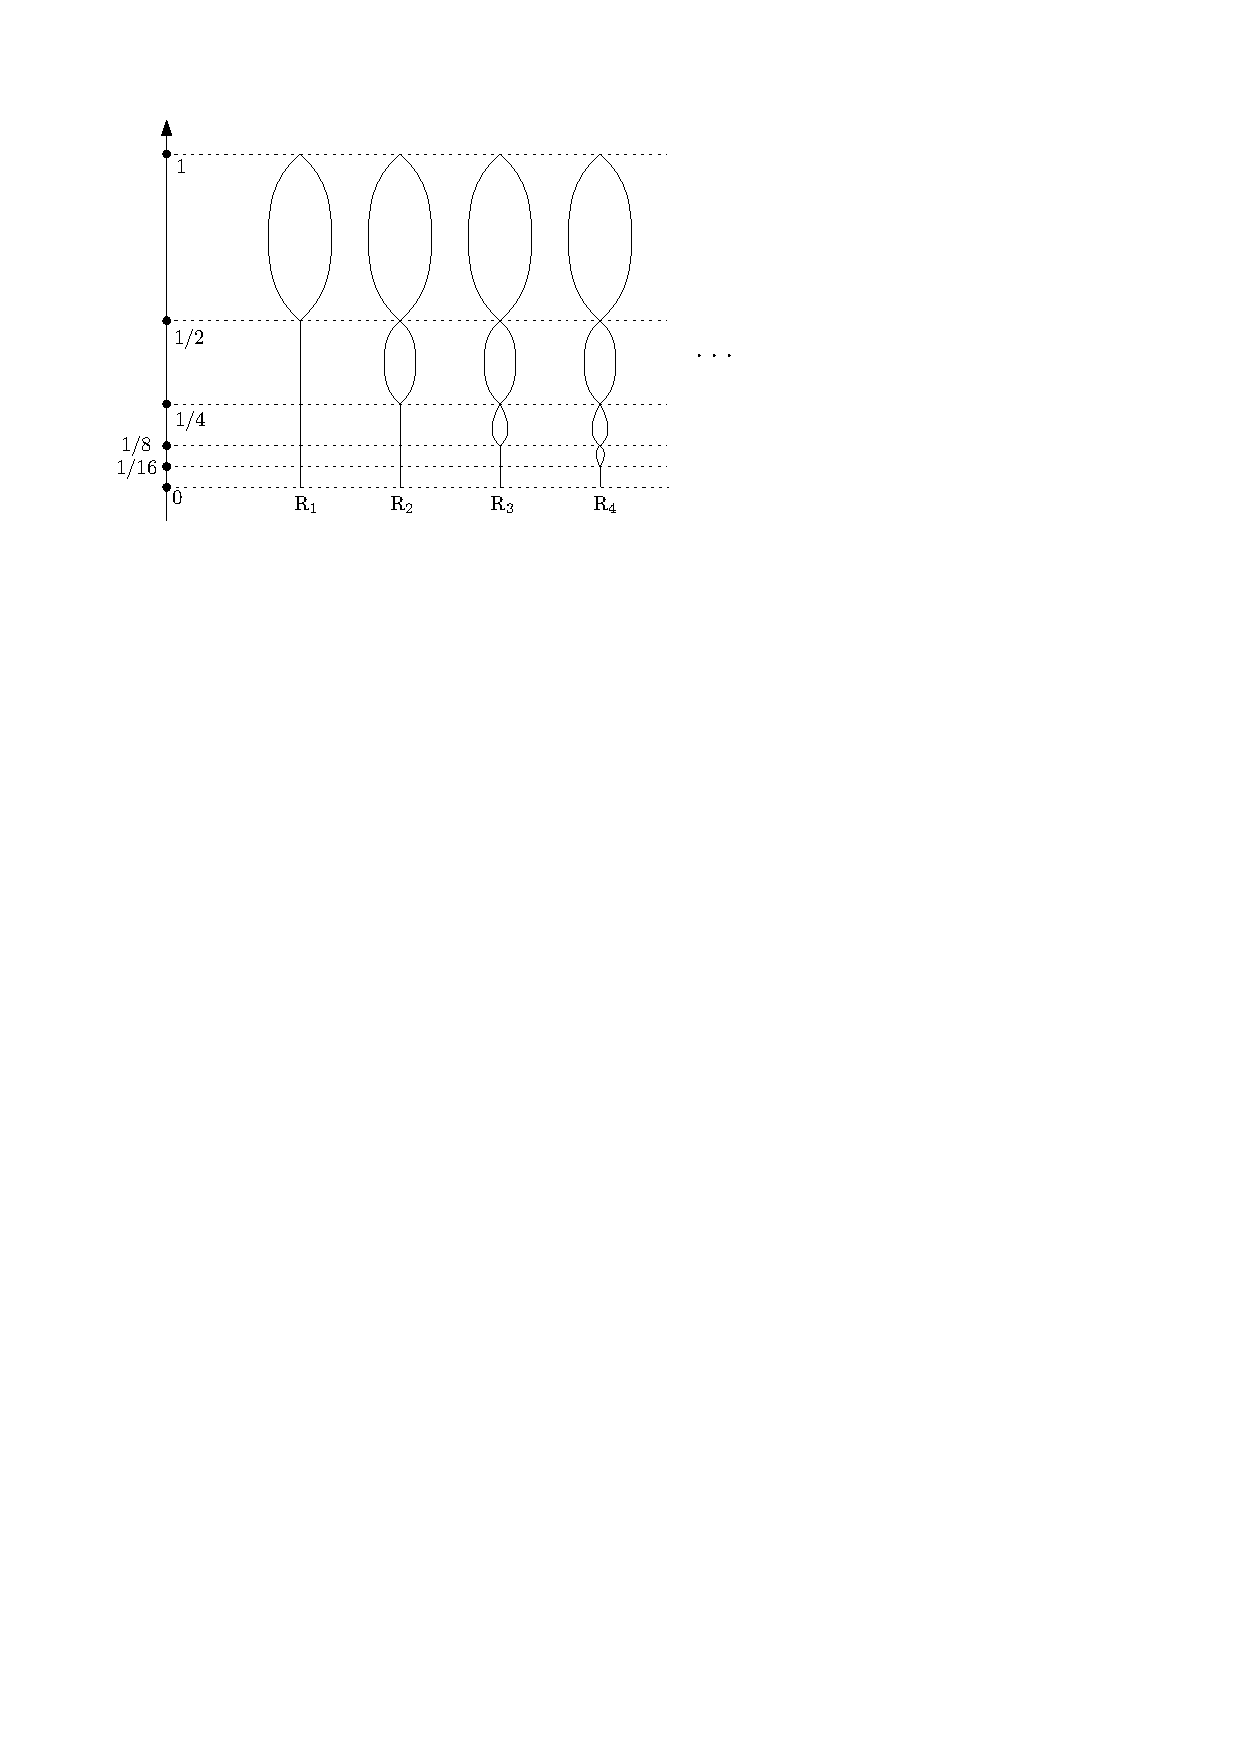
\includegraphics[width=7.5cm]{figures/CounterExampleCauchy}
  \caption[The space of Reeb graphs is not Cauchy]{\label{fig:ce}
  A sequence of Reeb graphs that is Cauchy but that does not converge in $\RS$ because the number of critical values goes to $+\infty$.
  Indeed, each $\Reeb_n$ has $n+2$ critical values.}
  \end{figure}

\item {\bf Is $\RS$ an Alexandrov space?} Provided shortest paths
  exist in $\RS$ (or in some subspace thereof), one can investigate whether
  the intrinsic curvature is bounded, either from above or from
  below.  This is interesting because barycenters in metric spaces
  with bounded curvature enjoy many useful
  properties~\cite{Ohta12}, and they can be approximated
  effectively in practice~\cite{Ohta09}.

\item {\bf Can the local equivalence be extended to general metric
  spaces?} We have reasons to believe that our local equivalence
  result can be used to prove similar results for more general 
  classes of metric spaces than Reeb graphs. If true, this 
  would shed new light on inverse problems in persistence theory.

\end{itemize}  

%\bibliographystyle{plain}
%\bibliography{biblio}